



\newpage

%----------------------------------------------------------------------------------------


%\section[Unveiling Network Effects][Effets de Réseaux]{Network effects unveiled by a macroscopic growth model}{Effets de Réseau révélés par un modèle de croissance macroscopique}
\section{Macroscopic growth model}{Modèle de croissance macroscopique}


\label{sec:interactiongibrat}


%----------------------------------------------------------------------------------------


Le dernier aspect de la Théorie Evolutive des Villes que nous proposons d'explorer, se positionne sur le plan thématique et sur le plan de la modélisation : l'étude des villes elles-mêmes et de leur interactions, par l'intermédiaire de modèles de simulation. Comme nous allons le voir, la plupart des modèles de systèmes de villes issus de la théorie évolutive se basent sur les interactions entre villes : cela nous permet une entrée directe dans notre problématique puisque celles-ci se font par l'intermédiaire des réseaux, qu'on pourra alors expliciter dans nos modèles.



\bpar{
We describe a simple spatial model of urban growth for systems of cities at the macroscopic scale, which combines direct interaction between cities and an indirect effect of physical network flows as population growth drivers. The model is parametrized on population data for the French system of cities between 1831 and 1999, which strong non-stationarity in correlation patterns suggest to apply the model on local time windows. The corresponding calibration of the model using genetic algorithms provide the evolution of interaction processes and network effects in time. Furthermore, the fit improvement when adding network module appears effective when controlling for additional parameters, what confirms the ability of the model to unveil network effects in the system of cities.
}{
Nous décrivons ainsi un modèle spatial simple de croissance urbaine pour les systèmes de villes à l'échelle macroscopique, qui combine les interactions directes entre les villes et un effet indirect des flux du réseau physique comme moteurs de la croissance de population. Le modèle est paramétré sur les données de population pour le système de villes français entre 1831 et 1999, dont la forte non-stationnarité des motifs de corrélation suggère d'appliquer le modèle sur des fenêtres temporelles locales. Les calibrations correspondantes du modèle par l'utilisation d'algorithmes génétiques fournit l'évolution des processus d'interaction et des effets de réseau dans le temps. De plus, l'amélioration de l'ajustement par l'ajout du module de réseau apparaît comme effectif lorsqu'on contrôle pour les paramètres supplémentaires, ce qui confirme la capacité du modèle à révéler des effets de réseau dans le système de villes.
}


\bpar{
In this section we aim at exploring further the assumption, central to Pumain's Evolutive Urban Theory, that spatial interactions between cities are significant drivers of their growth. More precisely, we consider both abstract interactions and flow interactions mediated through the physical networks, mainly transportation network. We extend existing models accordingly. Our contribution is twofold: (i) we show that very basic interaction models based on population only can be fitted to empirical data and that fitted parameter values are directly interpretable; and (ii) we introduce a novel methodology to quantify overfitting in models of simulation, as an extension of Information Criteria for statistical models, which applied to our calibrated models confirms that fit improvement is not only due to additional parameters, but that the extended model effectively capture more information on system processes. This will unveil network effects in an indirect way. We first review modeling approaches to urban growth based on spatial interactions.
}{
Dans cette section, nous visons à explorer plus en détail l'hypothèse, centrale à la Théorie Evolutive des Villes de \noun{Pumain}, selon laquelle les interactions spatiales sont des moteurs significatifs de leur croissance. Plus précisément, nous considérons à la fois les interactions abstraites et les interaction avec les flux portés par les réseaux physiques, principalement les réseaux de transport. Nous étendons les modèles existants de manière correspondante. Les apports de cette section consistent en deux points : (i) nous montrons que des modèles d'interaction très basiques basés uniquement sur la population peuvent être ajustés aux données empiriques et que les valeurs ajustées des paramètres sont directement interprétables ; et (ii) nous introduisons une nouvelle méthodologie pour quantifier l'overfitting dans les modèles de simulation, comme une extension de Critères d'Information pour les modèles statistiques, qui appliquée à nos modèles calibrés confirme que l'amélioration du fit n'est pas due seulement aux paramètres supplémentaires et donc artificielle, mais que le modèle étendu capture effectivement plus d'information sur les processus du système. Cela révèlera des effets de réseaux de manière indirecte. Nous précisons d'abord le contexte thématique dans lequel le modèle se placera et revoyons les approches de modélisation de la croissance urbaine basées sur les interactions spatiales.
}




\subsection{Spatial interaction models}{Modéliser la croissance	urbaine par les interactions spatiales}


\subsubsection{Models of Urban Growth}{Modèles de croissance urbaine}

\bpar{
Cities are paradoxically both unsustainable and source of negative externalities, but also the best chance to reach sustainability and resilience to climate change~\citep{glaeser2011triumph}. The dynamics of Urban Systems at a macroscopic scale, and more precisely drivers of urban growth, are crucial to be understood to meet these potentialities. A better knowledge of how cities differentiate, interact and grow is thus a relevant topic both for policy application and from a theoretical perspective. \cite{pumain2009innovation} suggests that cities are incubators of social change, their fate being closely linked to the one of societies. Various disciplines have studied models of urban growth with different objectives and taking diverse aspects into account. For example, Economics are still reluctant to include spatial interactions in the models~\citep{krugman1998space} but are extremely detailed on market processes, even for models in Economic Geography, whereas Geography focuses more on territorial specificities and interactions in space but will produce general conclusion with more difficulty. The example of this two disciplines shows how it is difficult to make bridges, as it needed exceptional efforts to translate from one to the other (as P. Hall did for Von Thunen work~\citep{taylor2016polymath}), and therefore how it is far from evident to grasp the complexity of Urban Systems in an integrated way.
}{
%Les villes sont de manière paradoxale à la fois non-soutenables et source d'externalités négatives, mais aussi la meilleure chance d'atteindre la soutenabilité et la résilience au changement climatique~\cite{glaeser2011triumph}.\comment[FL]{quel rapport avec la question de recherche ?}[(JR) aucun, c'est pour avoir une intro choc pour le papier - a supprimer ?] Les dynamiques des systèmes urbains à une échelle macroscopiques, et plus précisément les moteurs de la croissance urbaine, doivent nécessairement être compris pour atteindre ces objectifs.
Replaçons la présente démarche dans un contexte plus global de modélisation de la croissance urbaine\footnote{Qu'on comprend ici comme l'évolution dans le temps des villes, vue typiquement par l'évolution de leur population ou des activités économiques, et de leur distribution spatiale.}, notion plus générale que notre problématique précise. Elle nous permet ici toutefois de construire un premier modèle du point de vue de la Théorie Evolutive. Une bonne connaissance de la façon dont les villes se différencient, interagissent et croissent est ainsi un sujet pertinent à la fois pour les applications en termes de politiques et d'un point de vue théorique. \cite{pumain2009innovation} suggère que les villes sont l'incubateur du changement social, leur destin étant étroitement lié à celui des sociétés, et donc comme nous l'avons développé en Chapitre~\ref{ch:thematic}, de leurs territoires et de leurs réseaux. Diverses disciplines ont étudié des modèles de croissance urbaine avec différents objectifs et prenant en compte des aspects variés. Par exemple, l'économie est toujours prudente à inclure les interactions spatiales dans les modèles~\cite{krugman1998space}, le prenant en compte de façon très simplifiée même en économie géographique, mais produisant des modèles extrêmement détaillés en termes de processus de marché. Au contraire, la géographie se concentre plus sur les spécificités territoriales et les interactions dans l'espace mais produira des conclusions générales avec plus de difficulté~\cite{marchionni2004geographical}. L'exemple de ces deux disciplines montre comment il est difficile de créer des ponts, comme il a fallu des efforts exceptionnels pour effectuer des traductions de l'une à l'autre (comme \noun{P. Hall} le fit avec le travail de \noun{Von Thünen}~\cite{taylor2016polymath}), et ainsi comment il est loin d'être évident de capturer la complexité des systèmes urbains de manière intégrée.
}


\bpar{
The simplest model to explain urban growth, the Gibrat model, that assumes random growth rates, has been shown by~\cite{gabaix1999zipf} to asymptotically produce the expected rank-size law (Zipf's law) for system of cities which is considered as one of the most regular stylized facts, at least in its generalized scaling law formulation~\citep{nitsch2005zipf}. Explaining urban scaling laws is closely related to the understanding of urban growth, as \cite{bettencourt2008large} suggests that these reflect underlying universal processes and that all cities are scaled version of each other. This approach however does not reflect the complex relation between economic agents for which~\cite{storper2009rethinking} advocates.
}{
Le modèle le plus simple pour expliquer\footnote{C'est à dire essayant de traduire et d'inclure ses processus fondamentaux et de reproduire ses faits stylisés.} la croissance urbaine, le modèle de Gibrat, qui suppose des taux de croissance aléatoires, a été montré par~\cite{gabaix1999zipf} produisant asymptotiquement la loi rang-taille (loi de Zipf) attendue pour les systèmes de ville et qui est considérée comme l'un des faits stylisés les plus réguliers, au moins dans sa formulation généralisée sous forme de loi d'échelle~\cite{nitsch2005zipf}. Expliquer les lois d'échelles urbaines est étroitement lié à la compréhension de la croissance urbaine, comme \cite{bettencourt2008large} suggère que celles-ci reflètent des processus universels sous-jacents et que les propriétés individuelles des villes s'expliquent par un passage à l'échelle. Cette approche reflète cependant peu les relations complexes entre agents économiques pour lesquelles~\cite{storper2009rethinking} se positionnent.
}


\bpar{
 Using a bottom reconstruction of urban areas using dynamical microscopic population data, \cite{rozenfeld2008laws} shows indeed that positive deviations to the rank-size law systematically exist, and that these must be an effect of spatial interaction between urban areas. Complexity approaches are good candidates to integrate these into models. \cite{andersson2006complex} introduce for example a model of urban economy as a growing complex network of relations. The Evolutive Urban Theory, introduced by~\cite{pumain1997pour}, focuses on cities as co-evolving entities and produces explanations for growth at the system of cities level. \cite{pumain2006evolutionary} shows that scaling laws could be due to functional differentiation and diffusion of innovation between cities. The positioning regarding universality of laws is more moderate than Scaling theories, as \cite{pumain2012urban} highlights that ergodicity can difficultly be assumed in the frame of complex territorial systems. One crucial feature of this paradigm is the importance of interactions between agents, generally the cities, to produce the emergent patterns at the scale of the system. \cite{pumain2013theoretical} has investigated the advantages of Agent-based models compared to more classical equation systems, and this methodological aspect is in accordance with the theoretical positioning, as it allows to take into account the heterogeneity of possible interactions, the geographical particularities, and to naturally translate emergence between levels and render multi-scale patterns.
}{
Par l'utilisation d'une reconstruction par le bas des zones de population contigue via des données microscopiques dynamiques de population, \cite{rozenfeld2008laws} montrent en effet que des déviations aux tailles attendues par la loi rang-taille existent systématiquement, celles-ci étant sous-estimées, ce qui est probablement un effet des interactions spatiales entre les aires urbaines. Les approches par la complexité sont de bon candidats pour intégrer celles-ci dans les modèles. \cite{andersson2006complex} introduit par exemple un modèle d'économie urbaine comme un réseau complexe de relations en croissance. La Théorie Evolutive Urbaine, introduite par~\cite{pumain1997pour}, se concentre sur les villes comme des entités en co-évolution et produit des explications pour la croissance au niveau du système de villes. \cite{pumain2006evolutionary} montrent que les lois d'échelles pourraient être dues à la différentiation fonctionnelle et la diffusion de l'innovation entre les villes. Les positionnement au regard de l'universalité des lois est plus modéré que les théories du \emph{Scaling} comme celle de~\cite{west2017scaling}, puisque \cite{pumain2012urban} souligne que l'ergodicité peut difficilement être prise pour acquise dans le cadre des systèmes complexes territoriaux. Un aspect crucial de ce paradigme est l'importance des interactions entre agents constituants du système, généralement les villes, qui produisent les motifs émergents à l'échelle supérieure. \cite{pumain2013theoretical} a investigué les avantages des modèles basés-agents comparé à des systèmes d'équations plus classiques, et cet aspect méthodologique est en accord avec le positionnement théorique, comme cela permet de prendre en compte l'hétérogénéité des interactions possibles, les particularités géographiques, et de traduire naturellement l'émergence entre les niveaux et rendre compte de motifs multi-échelles.
}


\subsubsection{Urban Growth and Spatial Interaction}{Croissance Urbaine et Interactions Spatiales}

\bpar{
First of all, we must precise that we consider only models at the macro-scale, ruling out the numerous and rich approaches at the mesoscopic scale, that include for exemple Cellular Automata models, models of Urban Morphogenesis or Land-use change models. We also naturally rule out economics models that do not include explicitly spatial interactions. Several models of Urban Growth at the macro scale have insisted on the role of space and spatial interactions. \cite{bretagnolle2000long} proposed a spatial extension of the Gibrat model. The gravity-based interaction model that~\cite{sanders1992systeme} use to apply concept of Synergetics to cities is also close to this idea of interdependent urban growth, contained physically in the phenomenon of migration between cities. A more refined extension with economic cycles and innovation waves was developed by~\cite{favaro2011gibrat}, yielding a system dynamics version of the core of Simpop models~\citep{pumain2012multi}.
}{
Dans un premier temps, nous devons préciser que nous considérons seulement les modèles à l'échelle macroscopiques, ne considérant pas les nombreuses approches très riches à l'échelle mesoscopique, qui incluent par exemple les modèles à automates cellulaires, les modèles de morphogenèse urbaine que nous aborderons en Chapitre~\ref{ch:morphogenesis} ou les modèles de changement d'usage du sol. Nous excluons aussi naturellement les modèles économiques qui n'incluent pas explicitement les interactions spatiales. Un certain nombre de modèles de croissance urbaine à l'échelle macroscopique ont insisté sur le rôle de l'espace et des interactions spatiales, que nous allons illustrer par la suite. \cite{bretagnolle2000long} a proposé une extension spatiale du modèle de Gibrat. Le modèle d'interaction basé sur la gravité que \cite{sanders1992systeme} utilise pour appliquer les concepts de la Synergétique aux villes est également proche de cette idée de croissance urbaine interdépendante, contenue physiquement dans le phénomène de migration entre les villes. Une extension plus raffinée avec des cycles économiques et des vagues d'innovation a été développé par~\cite{favaro2011gibrat}, fournissant une version du coeur des modèles Simpop~\cite{pumain2012multi} en termes de systèmes dynamiques.
}

\bpar{
This family of models have started with a toy-model based on economic interactions between cities as agents, that yield hierarchical patterns at the scale of the system~\citep{sanders1997simpop}. Later, the Simpop2 model, still based on distance interaction for commercial exchanges, including successive innovation waves, unveiled structural differences between the European and the US Urban Systems~\citep{bretagnolle2010comparer}. The SimpopLocal model~\citep{pumain2017simpoplocal} is used to show the emergence of initial settlement patterns. The Marius model~\citep{cottineau2014evolution} couples population and economic growth with cities interaction, allowing to accurately reproduce real trajectories on the former Soviet Union after calibration with multi-modeling of processes.
}{
La famille des modèles Simpop a été développée en symbiose avec la Théorie Évolutive des villes, avec la caractéristique principale de modèles basés sur les agents prenant en compte l'interaction spatiale. Les modèles ont été progressivement raffiné, et spécifiés pour divers cas d'étude. Nous pouvons  donner un aperçu chronologique d'un échantillon de ceux-ci. Cette famille de modèles a commencé avec un modèle stylisé basé sur les interactions économiques entre les villes comme agents, qui produit des motifs de hiérarchie à l'échelle du système~\cite{sanders1997simpop}. Plus tard, le modèle Simpop2, toujours basé sur l'interaction en fonction de la distance pour les échanges commerciaux, incluant les vagues successives d'innovation, a dévoilé des différences structurelles entre le système de villes Européen et le système aux Etats-Unis~\cite{bretagnolle2010comparer}. Le modèle SimpopLocal~\cite{pumain2017simpoplocal} est utilisé pour montré l'émergence des motifs initiaux d'établissement humains. Enfin, le dernier modèle similaire en date, le modèle Marius~\cite{cottineau2014evolution} couple la croissance de la population et économique avec les interactions entre les ville, permettant de reproduire assez fidèlement les trajectoires réelles (au sens de l'erreur carré moyenne dans le temps sur l'ensemble des populations) sur l'ancienne Union Soviétique après calibration avec multi-modélisation des processus.
}


%%%%%%%%%%%%%%%%%%%%%%%%
\subsubsection{Urban Growth and Transportation Networks}{Croissance Urbaine et Réseaux de Transports}


Nous situons ici l'aperçu que nous venons de donner en regard des modèles s'intéressant aux interactions entre territoires et réseaux que nous avons amplement revu en Chapitre~\ref{ch:modelinginteractions}.

\bpar{
Under similar assumptions of previously reviewed models, the inclusion of transportation networks has been rarely pursued, contrary to the mesoscopic scale at which relations between networks and territories have been widely studied by Luti models for example~\citep{chang2006models}. Network growth models~\citep{xie2009modeling}, prolific in Economics and Physics, can not be utilized to explain urban growth.
}{
Dans des hypothèses similaires aux modèles précédemment revus, l'inclusion des réseaux de transports a été rarement poursuivie, contrairement à l'échelle mesoscopique à laquelle les relations entre réseaux et territoires ont été largement étudiées par les modèles Luti par exemple~\cite{chang2006models}. Les modèles de croissance de réseau~\cite{xie2009modeling}, prolifiques en économie et physique, ne peuvent pas être utilisés pour expliquer la croissance urbaine.
}

\bpar{
\cite{bigotte2010integrated} studies an optimization model for network design combining the effects of urban hierarchy and of transportation network hierarchy. \cite{baptiste1999interactions} has modeled dynamical interplay between network links capacity and city growth on a subset of French city system. The SimpopNet model~\citep{schmitt2014modelisation} goes a step further in modeling the co-evolution between cities and transportation networks, as it allows new network links to be created in time. These examples shows the difficulty of coupling these two aspects of urban systems in models of growth, and we will for this reason take into account network effects in a simplified way as detailed further.

}{
\cite{bigotte2010integrated} étudie un modèle d'optimisation pour la conception du réseau combinant les effets de la hiérarchie urbaine et de la hiérarchie du réseau de transport. \cite{baptiste1999interactions} a modélisé l'intrication dynamique entre la capacité des liens du réseau et la croissance des villes sur un sous-ensemble du système de villes français. Le modèle SimpopNet~\cite{schmitt2014modelisation} va un pas plus loin dans la modélisation de la co-évolution entre les villes et les réseaux de transport, puisqu'il permet que de nouveaux liens soit créés dans le temps. Ces exemples montrent la difficulté de coupler ces deux aspects des systèmes urbains dans les modèles de croissance, et nous prendrons en compte pour cette raison les effets de réseau d'une manière simplifiée comme nous le détaillerons par la suite.
}

%\comment[FL]{cela devrait etre dans le chapitre 2}[(JR) j'en ai deja parlé ; ca ne marche pas là en mini etat de l'art local pour bien situer le modèle ?][(FL) je maintiens ma remarque ; sauf si lien fort avec la suite][(JR) oui lien fort : situer la biblio urban growth par rapport aux modeles reseaux et territoires]


\bpar{
The rest of this section is organized as follows : our model is introduced and formally described in next section; we then describe results obtained through exploration and calibration of the model on data for French cities, in particular the unveiling of network effects significantly influencing growth processes thanks to a novel methodology introduced. We finally discuss the implications of these results.
}{
La suite de cette section est organisée de la manière suivante: nous introduisons notre modèle macroscopique et le décrivons de manière formelle ; puis nous donnons les résultats obtenus par l'exploration et la calibration du modèle sur les données pour les villes françaises, plus particulièrement la révélation d'effets de réseaux influençant de manière significative les processus de croissance, grâce à une nouvelle méthodologie spécifiquement introduite. Nous discutons finalement les implications de ces résultats.
}

Le modèle de croissance à l'échelle macroscopique introduit et étudié en détails ici servira alors de brique élémentaire pour la construction des modèles de co-évolution que nous mènerons par la suite.





%%%%%%%%%%%%%%%%%%%%%%%%%
\subsection{Model and Results}{Modèle et Résultats}




%%%%%%%%%%%%%%%%%%%%%%%%%
\subsubsection{Model Description}{Description du modèle}




\paragraph{Rationale}{Hypothèses}


\bpar{
Some confusion may arise when surveying at stochastic and deterministic models of urban growth. To what extent is a proposed model ``complex'' and is the simulation of stochasticity necessary ? Concerning Gibrat model and most of its extensions, independence assumptions and linearity produce a totally predictable behavior and thus not complex in the sense of exhibiting emergence, in the sense of weak emergence~\citep{bedau2002downward}. In particular, the full distribution of random growth models can be analytically determined at any time~\citep{gabaix1999zipf}, and in the case of studying only first moment, a simple recurrence relation avoids to proceed to any Monte-Carlo simulation. Under these assumptions, it is natural to work with a deterministic model, as it is done for example for the Marius model~\citep{cottineau2014evolution}. We will work under that hypothesis, capturing complexity through non-linearity. We work on simple territorial systems assumed as regional city systems, in which cities are basic entities. The time scale corresponds to the characteristic scale associated to this spatial scale, i.e. around one or two centuries. Spatial interactions will be captured through gravity-type interactions, this formulation having the advantage of being simple and of capturing the first law of Tobler, namely that interaction strength fades with distance. Other approaches introduced recently perform similarly at this scale~\citep{masucci2013gravity}.
}{
Une confusion peut régner lorsqu'on s'intéresse aux modèle stochastiques et déterministes de croissance urbaine. Dans quelle mesure un modèle proposé est-il ``complexe'' et la simulation de la stochasticité nécessaire ?  Concernant le modèle de Gibrat et la plupart de ses extensions, les hypothèses d'indépendance et la linéarité produisent un comportement totalement prédicable, ce qui ne les rend pas complexes au sens d'exhiber une émergence faible~\cite{bedau2002downward}. En particulier, la distribution complète des modèles de croissance aléatoire peut être déterminée analytiquement à tout instant~\cite{gabaix1999zipf}, et dans le cas de l'étude du premier moment seulement, une simple relation de récurrence évite de procéder à toute simulation de Monte-Carlo. Sous ces hypothèses, il est raisonnable de travailler avec un modèle déterministe, comme il est fait par exemple pour le modèle Marius~\cite{cottineau2014evolution}\footnote{Le modèle Marius introduit par \cite{cottineau2014evolution} pour l'évolution des villes en ex-Union soviétique, lie les variables économiques et de population à l'échelle de villes en prenant en compte leurs interactions. Le modèle a été conçu dans une perspective de modélisation incrémentale et divers processus peuvent être considérés.}. Nous travaillerons sous cette hypothèse, capturant la complexité par la non-linéarité. Nous travaillons sur des systèmes territoriaux simples supposés comme des systèmes de villes régionaux, dans lesquels les villes sont les entités de base. Nous avons ainsi de l'ordre d'une centaine de villes, et les territoires intermédiaires ne sont pas pris en compte. L'échelle de temps correspond à l'échelle caractéristique associée à cette échelle spatiale, i.e. autour d'un ou deux siècles. Les interactions spatiales sont capturées par des interactions de type gravitaire, cette formulation ayant l'avantage de la simplicité et de capturer la première loi de Tobler, c'est à dire que la force d'interaction décroit avec la distance. Ce choix n'a a priori pas une influence fondamentale sur le comportement du modèle, puisque d'autres approches différentes du paradigme gravitaire comme le modèle de radiation, introduites plus récemment, ont des performances similaires à cette échelle~\cite{masucci2013gravity}.
}

\paragraph{Model description}{Description}

\bpar{
We consider on a deterministic extension of the Gibrat model, what is equivalent to consider only expectancies in time. Let $\vec{P}(t)=(P_i(t))_{1\leq i\leq n}$ be the population of cities in time. Under Gibrat independence assumptions, we have $\Covb{P_i(t)}{P_j(t)}=0$. A linear extended version would write $\vec{P}(t+1)=\mathbf{R}\cdot \vec{P}(t)$ where $\mathbf{R}$ is an independent random matrix of growth rates (a scalar times identity in the original case). It yields directly thanks to the independence assumption that $\Eb{\vec{P}(t+1)}=\Eb{\mathbf{R}}\cdot\Eb{\vec{P}}(t)$.
}{
Nous considérons une extension déterministe du modèle de Gibrat, ce qui est équivalent à considérer seulement les espérances des populations dans le temps et ne plus simuler des trajectoires aléatoires. Soit $\vec{P}(t)=(P_i(t))_{1\leq i\leq n}$ le vecteur des populations des villes dans le temps. Sous les hypothèses d'indépendance de Gibrat\footnote{On rappelle que le modèle de Gibrat suppose des taux de croissance aléatoires indépendants : $P_i (t+1) = r\cdot P_i(t)$.}, nous avons $\Covb{P_i(t)}{P_j(t)}=0$, c'est à dire que les villes ne s'influencent pas mutuellement dans leur processus de croissance. Une version étendue linéaire du modèle de Gibrat s'écrirait alors
\[
\vec{P}(t+1)=\mathbf{R}\cdot \vec{P}(t)
\]
où $\mathbf{R}$ est une matrice aléatoire indépendante de taux de croissance (l'identité à un scalaire près dans le cas original). Cela conduit directement grâce à l'hypothèse d'indépendance que $\Eb{\vec{P}(t+1)}=\Eb{\mathbf{R}}\cdot\Eb{\vec{P}(t)}$.
}

% \comment[FL]{pourquoi E(R) et pas R, autrement dit: pourquoi R est elle aleatoire ?}[(JR) hypothese de base de Gibrat $\rightarrow$ detailler plus Gibrat ?] 


\bpar{
We generalize this linear relation to a non-linear relation that allows to be more consistent with model interpretation and more flexible. Denoting $\vec{\mu}(t)=\Eb{\vec{P}(t)}$, we take $\vec{\mu}(t+1)=\Delta t\cdot f(\vec{\mu}(t))$. Note that in that case, stochastic and deterministic versions are not equivalent anymore, precisely because of the non-linearity, but we stick to a deterministic version for the sake of simplicity. The specification of the interdependent growth rate is given by
}{
Nous généralisons cette relation linéaire à une relation non-linéaire qui permet d'être plus cohérent avec les interprétations du modèle et plus flexible. Notant $\vec{\mu}(t)=\Eb{\vec{P}(t)}$, nous généraliserons cette relation avec une fonction donnée $f$ et un pas de temps quelconque $\Delta t$, sous la forme 
\[
\vec{\mu}(t+\Delta t)=\Delta t\cdot f(\vec{\mu}(t))
\]
Il faut noter que dans ce cas, les versions stochastiques et déterministes ne sont plus équivalentes, précisément à cause de la non-linéarité, mais nous gardons une version déterministe pour rester simple. La spécification des taux de croissance interdépendants est donnée par
}



\begin{equation}
f(\vec{\mu}) = (1+r_0)\cdot \mathbf{Id}\cdot \vec{\mu} + \mathbf{G}\left(\vec{\mu}\right)\cdot \vec{1} + \vec{N}\left(\vec{\mu}\right)
\label{eq:interactiongibrat:model}
\end{equation}

\bpar{
where $\vec{1}$ is the column vector full of ones, and $\mathbf{G} = G_{ij} = w_G\cdot \frac{V_{ij}}{<V_{ij}>}$ such that the interaction potential $V_{ij}$ follows a gravity-type expression given by, with $d_{ij}$ distance between $i$ and $j$ (euclidian or network distance),
}{
où  $\vec{1}$ est le vecteur colonne unité, et $\mathbf{G} = G_{ij} = w_G\cdot \frac{V_{ij}}{<V_{ij}>}$ est le terme d'interaction directe, de telle façon que le potentiel d'interaction $V_{ij}$ suit une expression de type gravitaire donnée par, avec $d_{ij}$ distance entre $i$ et $j$ (distance euclidienne ou distance de réseau),
}

\begin{equation}
V_{ij} = \left(\frac{\mu_i\mu_j}{\left(\sum_k{\mu_k}\right)^2}\right)^{\gamma_G}\cdot \exp{\left(-d_{ij}/d_G\right)}
\end{equation}

\bpar{}{
où $\gamma_G$ est un exposant de hiérarchie des interactions par rapport aux populations, $d_G$ un paramètre de décroissance donnant la distance typique d'interaction, et $w_G$ est le poids relatif des interactions directes.
}


\bpar{
The network effect term $\vec{N}$ is given by $N_{i} = w_N \cdot \frac{W_i}{<W_i>}$ where the network flow potential $W_i$ reads
}{
Le dernier terme capture un effet de réseau : $\vec{N}$ est donné par $N_{i} = w_N \cdot \frac{W_i}{<W_i>}$ où le potentiel du flux de réseau $W_i$ suit
}

%\comment[FL]{jusqu'a present on ne se posait pas la question : a amener}

\begin{equation}
W_{i} = \sum_{k < l} \left(\frac{\mu_k\mu_l}{\left(\sum_j\mu_j\right)^2}\right)^{\gamma_N} \cdot \exp{\left(-d_{kl,i}/d_N\right)}
\end{equation}

\bpar{
where $d_{kl,i}$ is the distance of city $i$ to the shortest path between $k,l$ computed in the geographical space, which can be through a transportation network or in an impedance field of the euclidian space. All seven model parameters are detailed below.
}{
où $d_{kl,i}$ est la distance de la ville $i$ au plus court chemin entre $k,l$ calculé dans l'espace géographique, qui peut être par un réseau de transport ou dans un champ d'impédance dans l'espace euclidien. Les paramètres $\gamma_N$, $d_N$ et $w_N$ sont analogues à ceux pour l'interaction directe. Les septs paramètres du modèle sont détaillés ci-dessous et récapitulés en Table~\ref{tab:interactiongibrat:parameters}. Précisons d'abord la logique de cette formulation.
}


\bpar{
The first component is the pure Gibrat model, that we obtain by setting the weights $w_G = w_N = 0$. The second component captures direct interdependencies between cities, under the form of a separable gravity potential such as the one used in~\cite{sanders1992systeme}. The rationale for the third term, aimed at capturing network effects by expressing a feedback of network flow between cities $k,l$ on the city $i$. Intuitively, a demographic and economic flow physically transiting through a city or in its surroundings is expected to influence its development (through intermediate stops e.g.), this effect being of course dependent on the transportation mode since a high speed line with few stops will skip most of the traversed territories. Note that we don't use exactly gravity flows in the network term, since there is no decay of interactions generating flows with distance, but a decay of the effect of the flow as a distance to the network: it is equivalent to assuming long-range use of the network on average in time, and is this way complementary to the first gravity term.
}{
Le premier terme de l'équation est le modèle de Gibrat seul, qui est obtenu en fixant les poids $w_G = w_N = 0$. La deuxième composante capture les interdépendances directes entre les villes, sous la forme d'un potentiel gravitaire séparable comme celui utilisé dans~\cite{sanders1992systeme}. La logique du troisième terme, qui a pour but de capturer l'effet de réseau en exprimant une rétroaction des flux du réseau entre les villes $k,l$ sur la ville $i$. Intuitivement, un flux démographique et économique transitant physiquement par une ville ou dans son voisinage est attendu d'avoir une influence sur son développement (par des arrêts intermédiaires e.g.), cet effet étant bien sûr dépendant du mode de transport puisqu'une ligne à grande vitesse avec peu d'arrêts ignorera la majorité des territoires traversés. Notons que nous n'utilisons pas exactement les flux gravitaires dans le terme de réseau, puisqu'il n'y a pas de décroissance des interactions générant les flux avec la distance, mais une décroissance de l'effet du flux en fonction de la distance au réseau. Cela est équivalent à supposer une utilisation du réseau sur de très longues portées en moyenne dans le temps, puisque le terme d'attenuation tend vers 1 si le paramètre de décroissance tend vers l'infini, ce qui est ainsi complémentaire au premier terme de gravité.
}



\paragraph{Model Parameter Space}{Espace des paramètres}


\bpar{
We give in Table~\ref{tab:interactiongibrat:parameters} the description of model parameters, detailing the associated processes and parameter ranges. Both direct interaction and second order network flows effect have the same structure, namely separability between effect of distance and population influence, an exponential decay parameter and a hierarchy parameter expressing the inequality of contribution depending on cities relative sizes: the highest the exponent, the more contribution of smaller cities will be negligible regarding larger cities. We propose to interpret the distance decay parameter the following way. Let fix an arbitrary fraction $\alpha$ and typical spatial ranges for a local urban system $d_L$ and for a long range urban system $d_R$, consider a city $i$ and two neighbors $j,j'$ with same population $\mu_j=\mu_j'$, at distances $d_L$ and $d_R$ of $i$ respectively. If we want to answer the question to what distance difference is equivalent an attenuation of $\alpha$ of the interaction potential with $i$, we obtain $d_L - d_R = -d_G\cdot \ln \alpha$. Therefore, $d_G$ is exactly the proportionality coefficient answering this intuitive request. Finally, we will consider only positive weights $w_G$ and $w_N$, to follow empirical observations as detailed below. Numerical values for the weights will be given normalized by number of cities implied in the process, i.e. ${w'}_G = w_G / n$ and ${w'}_N = w_N / (n (n-1) / 2)$.
}{
Nous donnons en Table~\ref{tab:interactiongibrat:parameters} la description des paramètres du modèle, détaillant les processus associés et les bornes des paramètres. Les interactions directes et les effets au second ordre des flux du réseau ont tous deux la même structure, c'est à dire le caractère séparable de l'effet de la distance et de l'influence des populations, un paramètre de décroissance exponentielle et un paramètre de hiérarchie exprimant l'inégalité des contributions selon les tailles relatives des villes : plus l'exposant est grand, plus les contributions des petites villes seront négligeables au regard des grandes villes. Le paramètre de décroissance de la distance peut s'interpréter comme une distance caractéristique d'atténuation des interactions\footnote{Il est possible d'établir formellement son expression exacte. Fixons une fraction arbitraire $\alpha$ et des portées spatiales typiques pour un système urbain local $d_L$ et pour un système urbain à longue portée $d_R$, considérons une ville $i$ et deux voisines $j,j'$ de population égale $\mu_j=\mu_j'$, à des distances respectives $d_L$ et $d_R$ de $i$. Si on veut répondre à la question à quelle différence de distance est équivalent une atténuation de $\alpha$ du potentiel d'interaction avec $i$, nous obtenons $d_L - d_R = -d_G\cdot \ln \alpha$. Pour cela, $d_G$ est exactement le coefficient de proportionnalité répondant à ce questionnement intuitif.}. Finalement, nous ne considérerons que des poids positifs, pour suivre les observations empiriques comme détaillé ci-dessous. Les valeurs numériques pour les poids seront données normalisées par le nombre de villes impliquées dans le processus, i.e. ${w'}_G = w_G / n$ et ${w'}_N = w_N / (n (n-1) / 2)$.
}


%%%%%%%%%%%%%%%%%%%%%%%%
\begin{table}[ht]
\caption[Model Parameters summary][Espace des paramètres du modèle d'interaction]{Model Parameters summary\label{tab:parameters}}{\textbf{Espace des paramètres du modèle d'interaction.} Nous donnons le nom du paramètre et sa notation, le processus du modèle qui lui est associé, une interprétation possible, et son domaine typique de variation.\label{tab:interactiongibrat:parameters}}
%\vspace{-1cm}
\begin{tabular}{|l|l|l|l|l|}
\hline
Paramètre & Notation & Processus & Interpretation & Domaine\\
\hline
Taux de Croissance & $r_0$ & Croissance Endogène & Croissance Urbaine & $\left[ 0,1\right]$ \\
Poids gravitaire & $w_G$ & Interaction directe & Croissance maximale & $\left[ 0,1\right]$ \\
Gamma gravitaire & $\gamma_G$ & Interaction directe & Niveau de hiérarchie & $\left[ 0,+\infty\right]$ \\
Décroissance gravitaire & $d_G$ & Interaction directe & Portée d'interaction & $\left[ 0,+\infty\right]$ \\
Poids de la rétroaction & $w_N$ & Effet des flux & Croissance maximale & $\left[ 0,1\right]$ \\
Gamma de la rétroaction & $\gamma_N$ & Effet des flux & Niveau de hiérarchie & $\left[ 0,+\infty\right]$ \\
Décroissance de la rétroaction & $r_0$ & Effet des flus & Portée de l'effet & $\left[ 0,+\infty\right]$ \\
\hline
\end{tabular}
\end{table}
%%%%%%%%%%%%%%%%%%%%%%%%




\subsubsection{Data}{Données}

\bpar{
Our model is assumed as hybrid as it relies on semi-parametrization on real data. It could be possible to study it as a full toy-model, initial configuration and physical environment being constructed as synthetic data. We however aim at unveiling stylized facts on real data rather than on model behavior in itself, and setup therefore the model from the data we now describe.
}{
Le modèle est construit pour être hybride, car nous proposons de l'étudier sur une semi-paramétrisation par données empiriques. Il pourrait être possible de l'étudier comme un modèle complètement jouet, la configuration initiale et l'environnement physique étant construits comme données synthétiques. Nous visons cependant à révéler des faits stylisés sur des données réelles plutôt que sur le comportement du modèle en lui-même, et initialisons ainsi le modèle à partir des données que nous décrivons à présent.
}

\paragraph{Population data}{Données de population}


\bpar{
We work with the Pumain-INED historical database for French Cities~\citep{pumain1986fichier}, which give populations of \emph{Aires Urbaines} (INSEE definition) at time intervals of 5 years, from 1831 to 1999 (31 observations in time). The latest version of the database integrates Urban Areas, allowing to follow them on long time-period, according to Bretagnolle's long time cities ontology~\citep{bretagnolle:tel-00459720}, that constructs a functional definition of cities as entities with boundaries evolving in time. We work on the 50 bigger cities in 1999. We furthermore isolate periods of similar length excluding wars, obtaining 9 periods of 20 years on which semi-stationary in time fit of the model will be done. 
}{
Nous travaillons avec la base de données historique Pumain-INED pour les villes françaises~\cite{pumain1986fichier}, qui donne les populations des Aires Urbaines (définition de l'INSEE) à des intervalles de temps de 5 ans, de 1831 à 1999 (31 observations temporelles). La version la plus récente de la base de données intègre les aires urbaines, permettant de les suivre sur de longues périodes de temps, suivant l'ontologie de \noun{Bretagnolle} pour les villes sur le temps long~\cite{bretagnolle:tel-00459720}, qui construit une définition fonctionnelle des villes comme entités dont les limites évoluent dans le temps. Pour simplifier, nous travaillons avec les 50 plus grandes villes en 1999\footnote{Ce choix n'ayant que peu d'influence sur la majorité des trajectoires des villes puisque les petites villes influent peu dans les processus d'interaction. Il peut en avoir sur l'ajustement des villes ajoutées, mais notre objectif n'étant pas de reproduire fidèlement l'ensemble des trajectoires mais de comprendre le rôle du réseau, nous fixons ce seuil.}. Nous isolons de plus des périodes de longueur similaires excluant les guerres, obtenant 9 périodes\footnote{Qui sont précisément : 1831-1851, 1841-1861, 1851-1872, 1881-1901, 1891-1911, 1921-1936, 1946-1968, 1962-1982, 1975-1999.} de 20 ans sur lesquelles l'ajustement du modèle non-stationnaire dans le temps sera exécuté.
}

%\comment[FL]{Pumain-INED : est-ce une expression admise}[(JR) oui ca vient de Denise elle-même]

\paragraph{Physical flows}{Flux physiques}

\bpar{
As stated before, this modeling exercise focuses on exploring the role of physical flows, whatever the effective shape of the network. We choose for this reason not to use real network data which is furthermore not easily available at different time periods, and physical flows are assumed to take the geographical shortest path taking into account terrain slope. It avoids geographical absurdities such as cities with a difficult access having an overestimated growth rate. Using a 1km resolution Digital Elevation Model, we construct an impedance field of the form
}{
Comme rappelé précédemment, cet exercice de modélisation se concentre sur l'exploration du rôle des flux physiques, quelle que soit la forme effective du réseau. Nous choisissons pour cette raison de ne pas utiliser de vraies données de réseau qui sont de plus difficiles à obtenir à différentes périodes de temps, et nous supposons que les flux physiques prennent le plus court chemin géographique prenant en compte la pente du terrain. Cela évite des absurdités géographiques comme des villes difficilement accessibles ayant un taux de croissance surestimé. Utilisant le Modèle d'Elevation Numérique de l'IGN à la résolution 1km, nous calculons les plus courts chemins de manière standard~\cite{collischonn2000direction}, par la construction d'un champ d'impédance de la forme
}

\[
Z = \left(1 + \frac{\alpha}{\alpha_0}\right)^{n_0}
\]


\bpar{
where $Z$ is the impedance of links of the 1km grid network in which each cell is connected to its eight neighbors. $\alpha$ is the terrain slope computed with elevation difference between the two cells. We take fixed parameter values $\alpha_0 = 3$ (corresponding to approximatively the real world value of a 5\% slope) and $n_0 = 3$ which yielded more realistic paths than smaller values.
}{
où $Z$ est l'impédance des liens du réseau de la grille de 1km dans laquelle chaque cellule est connectée à ses huit voisins. $\alpha$ est la pente du terrain calculée avec la différence d'altitude entre les deux cellules. Nous prenons des valeurs des paramètres fixes $\alpha_0 = 3$ (correspondant approximativement à la valeur réelle d'une pente de 5\%) et $n_0 = 3$ ce qui donne des chemins plus réalistes que des valeurs significativement plus petites ou plus grandes\footnote{Plus précisément, on a validé ``à dire d'expert'', en inspectant visuellement les chemins entre quelques destinations typiques (incluant Paris-Lyon, Lyon-Marseille, Lyon-Bordeaux par exemple), pour $\alpha_0 = 2,3,4$. Pour $\alpha_0 = 4$, le chemin est généralement trop rectiligne et coupe à travers des relief évités par les grands axes ; pour $\alpha_0 = 2$ le chemin est trop sinueux au contraire. On a testé $n_0 = 2,3$, le deuxième étant également plus crédible. Une calibration précise de ces paramètres nécessiterait l'ajustement par rapport au réseau autoroutier par exemple, mais est hors de portée de cet exercice ici.}.
}


%%%%%%%%%%%%%%%%%%%%%%%%%
\subsubsection{Performance indicators}{Indicateurs de performance}
%\subsubsection{Model Evaluation}{Evaluation du modèle} 
%\comment[FL]{titre a revoir}

\bpar{
We work on an explanatory rather than an exploratory model. Therefore, indicators to evaluate model outputs are not directly linked to intrinsic properties of trajectories or obtained final states, but rather to a distance to the phenomenon we want to explain, i.e. the data. Given real population $p_i(t)$ (historical realizations of $P_i(t)$) and simulated expected populations $\mu_i(t)$ obtained with $\vec{\mu}(t_0) = \vec{p}(t_0)$ on a period of length $T$, we can evaluate two complementary aspects of model performance:
}{
Nous travaillons sur un modèle explicatif plutôt qu'un modèle exploratoire. Pour cette raison, les indicateurs pour évaluer les sorties du modèle ne sont pas directement liés aux propriétés intrinsèques des trajectoires ou des états finaux obtenus, mais plutôt à une distance au phénomène que l'on cherche à expliquer, i.e. les données. Etant donné des populations réelles $p_i(t)$ (réalisations historiques de $P_i(t)$) et les espérances simulées $\mu_i(t)$ obtenues par $\vec{\mu}(t_0) = \vec{p}(t_0)$ sur une période de longueur $T$, on peut évaluer deux aspects complémentaires de la performance du modèle :
}

\bpar{
\begin{itemize}
\item Overall model performance, given by logarithm of the mean-square error in space and time
\[
\varepsilon_G = \ln{\left(\frac{1}{T}\sum_t \frac{1}{n} \sum_i \left(p_i (t) - \mu_i (t) \right)^2\right)}
\]
\item Average local model performance, given by the mean-square error on logarithms
\[
\varepsilon_L = \frac{1}{T}\sum_t \frac{1}{n} \sum_i \left(\ln p_i(t) - \ln \mu_i (t)\right)^2
\]
\end{itemize}
}{
\begin{itemize}
\item Performance globale du modèle, donnée par le logarithme de l'erreur carrée moyenne dans l'espace et le temps
\[
\varepsilon_G = \ln{\left(\frac{1}{T}\sum_t \frac{1}{n} \sum_i \left(p_i (t) - \mu_i (t) \right)^2\right)}
\]
\item La performance locale moyenne, donnée par l'erreur carrée moyenne des logarithmes, comme proposé par~\cite{pumain2017incremental}
\[
\varepsilon_L = \frac{1}{T}\sum_t \frac{1}{n} \sum_i \left(\ln p_i(t) - \ln \mu_i (t)\right)^2
\]
\end{itemize}
}


\bpar{
Both are actually complementary, as using only $\varepsilon_G$ as it is generally done will focus only on larger cities and give poor results on medium-sized and small cities (for France only Paris will have reasonable fit as it strongly dominates other urban areas and cities). $\varepsilon_L$ allows therefore to take into account model performance in all cities simulated by the model.
}{
Les deux sont en fait complémentaires, puisqu'utiliser seulement $\varepsilon_G$ comme il est généralement fait se concentrera seulement sur les plus grandes villes et donnera des résultats mitigés sur les villes de taille moyennes et les petites villes (pour la France seul Paris aura une estimation raisonnable comme il domine fortement les autres aires urbaines et villes). $\varepsilon_L$ permet pour cela de prendre en compte la performance du modèle sur l'ensemble des villes simulées par le modèle.
}







%%%%%%%%%%%%%%%%%%%%%%%%%
\subsubsection{Results}{Résultats}



\paragraph{Stylized facts}{Faits stylisés}

\bpar{
Basic stylized facts can be extracted from such a database, as it has already been widely explored in the literature~\cite{guerin1990150}. We retrieve better fits of log-normal distributions of growth rates at all dates compared to normal fits, and also the fact that growth rates are mainly positive, on the cities we consider and when removing wars.
}{
Des faits stylisés typiques peuvent être extraits d'une telle base de données, comme il a été déjà largement été exploré dans la littérature~\cite{guerin1990150}. Nous retrouvons les meilleurs ajustements de distributions log-normales des taux de croissance à toutes les dates en comparaison à des distributions normales, et également le fait que les taux de croissance sont essentiellement positifs, sur les villes que nous considérons et en enlevant les guerres.
}


\bpar{
An interesting feature to look at in relation with our considerations on spatial interactions are correlations between time-series, and more particularly their variation as a function of distance. We consider 50 years overlapping time-windows to have enough temporal observation, finishing respectively in (1881,1906,1931,1962,1999), and estimate on each, for each couple of cities $(i,j)$, the correlation between log-returns $\hat{\rho}_{ij}=\rho\left[\Delta X_i, \Delta X_j\right]$ with a classical Pearson estimator, where $\Delta X_i = X_i(t) - X_i(t-1)$ and $X_i(t) = \ln\left(\frac{P_i(t)}{P_i(t_0)}\right)$. This method, used mainly in econophysics~\citep{mantegna1999introduction}, reveals dynamical interactions without being biased by sizes.
}{
Un aspect intéressant à examiner en relation avec nos considérations sur les interactions spatiales sont les corrélations entre les séries temporelles, et plus particulièrement leur variation en fonction de la distance. Nous considérons des fenêtres temporelles de 50 ans se superposant pour avoir assez d'observations temporelles, finissant respectivement en (1881,1906,1931,1962,1999) et estimons sur chacune, pour chaque couple de villes $(i,j)$, la corrélation entre les log-returns, que nous définissons par $\Delta X_i = X_i(t) - X_i(t-1)$ et $X_i(t) = \ln\left(\frac{P_i(t)}{P_i(t_0)}\right)$, est donnée par $\hat{\rho}_{ij}=\rho\left[\Delta X_i, \Delta X_j\right]$ avec un estimateur de Pearson classique. Cette méthode permet de révéler des interactions dynamiques sans être biaisée par les tailles~\cite{mantegna1999introduction}.
}

\bpar{
We show in Figure~\ref{fig:interactiongibrat:ts-correlations} the smoothed correlations curves as a function of distance, for each time period. First of all, the strong differences between each confirms the non-stationarity of growth rates over the whole time period, and justifies the use of local fit in time for the model. We can also interpret these patterns in terms of historical events for the system of city and the transportation network. System dynamic begins with a flat correlation in 1881, around 0.2, that could be spurious due to simultaneous similar growth for all cities. It then stays flat but goes to zero, witnessing strong differentiations in growth patterns between 1856 and 1906. After 1931, the effect of the distance is clear with decreasing curves, starting between 0.4 and 0.5. We postulate that this evolution must be partly linked to transportation network evolution: considering railway network for example~\citep{thevenin2013mapping}, the initial overall development may have fostered long range interactions flattening thus the correlation curves, whereas its maturation over time has conducted to the return of more classical interactions decreasing quickly with distance.
}{
Nous montrons en Figure~\ref{fig:interactiongibrat:ts-correlations} les courbes de corrélations lissées en fonction de la distance, pour chaque période temporelle. Tout d'abord, les fortes différentes entre chaque confirme la non-stationnarité des taux de croissance sur l'ensemble de la période temporelle, et justifie l'utilisation d'ajustements locaux dans le temps pour le modèle. Nous pouvons aussi interpréter ces motifs en termes d'événements historiques pour le système de villes et le réseau de transport. La dynamique du système commence par une corrélation plate en 1881, autour de 0.2, qui pourrait être fortuite à cause de croissance similaire simultanée pour toutes les villes. Elle reste ensuite plate mais tend vers 0, témoignant de fortes différentiations dans les motifs de croissance entre 1856 et 1906. Après 1931, l'effet de la distance est clair avec des courbes décroissantes, commençant entre 0.4 et 0.5. Nous postulons que cette évolution doit être partiellement liée à l'évolution du réseau de transport : en considérant le réseau ferré par exemple~\cite{thevenin2013mapping}, le développement initial global a pu encourager des interactions à longue portée rendant ainsi les courbes de corrélation plates, tandis que sa maturation dans le temps a conduit au retour d'interactions plus classiques décroissant rapidement avec la distance.
}


%%%%%%%%%%%%%%%%%%%%%%%%%
\begin{figure}
%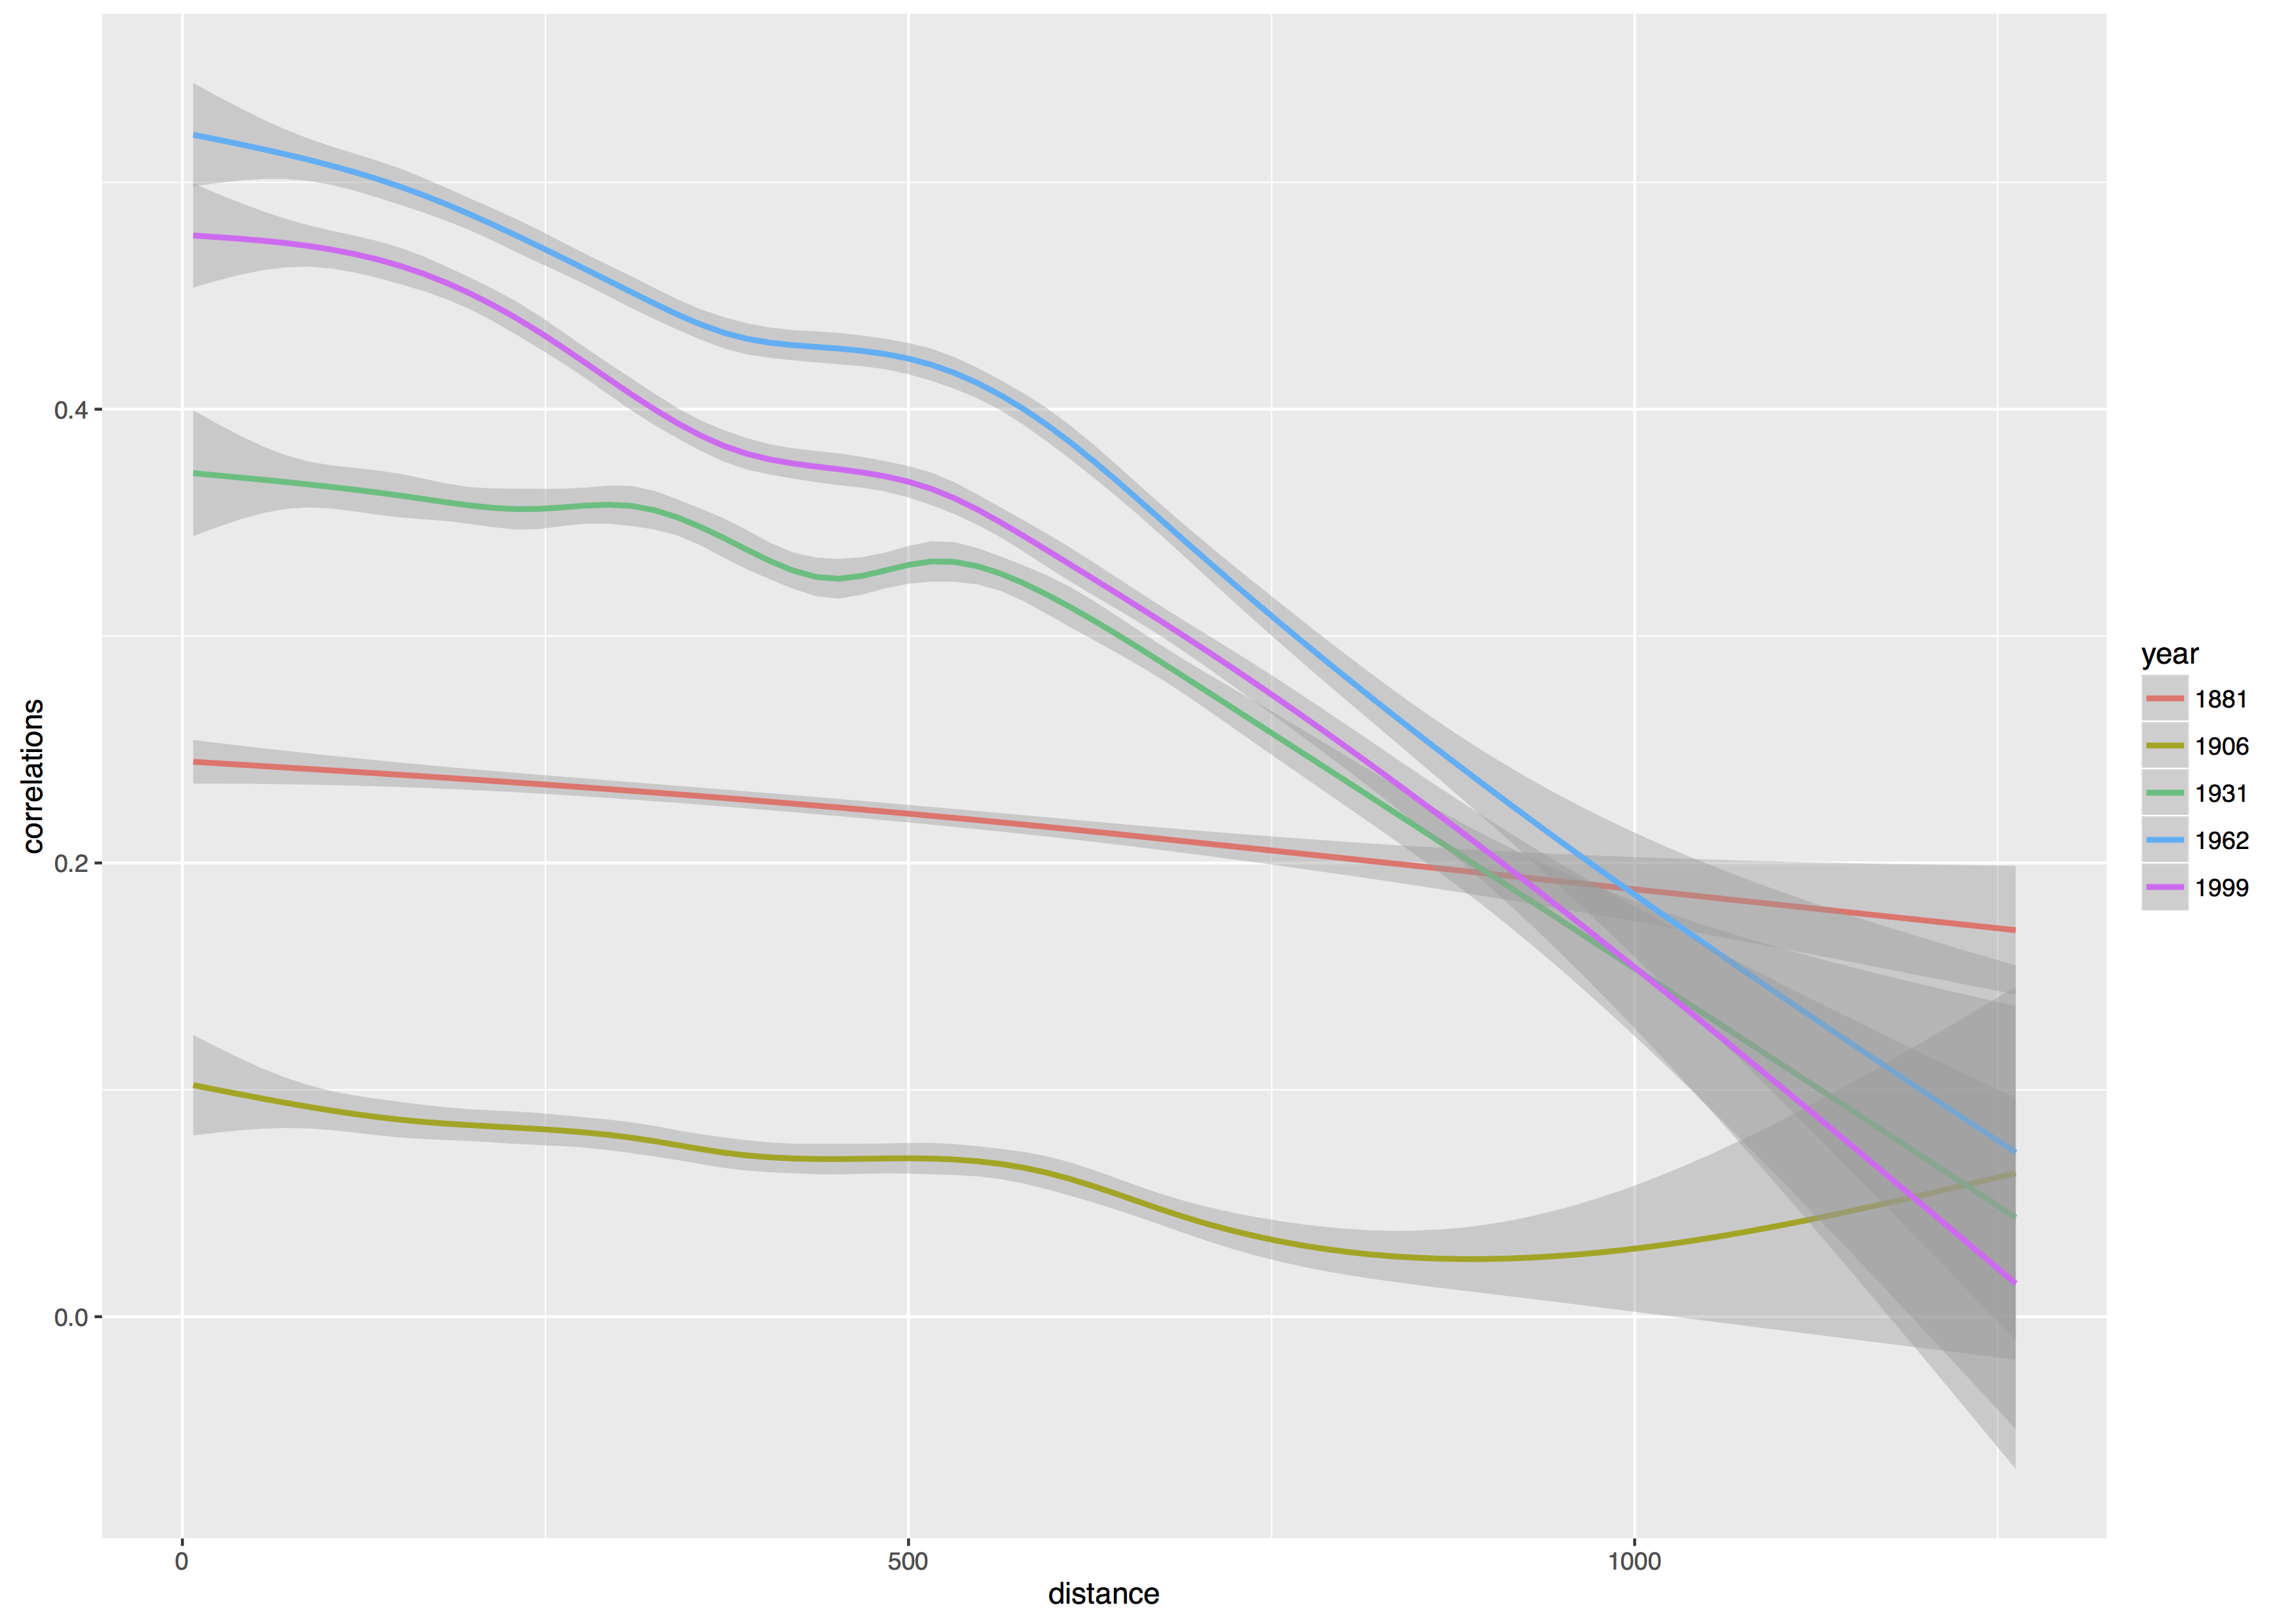
\includegraphics[width=\linewidth]{Figures/InteractionGibrat/Fig1}
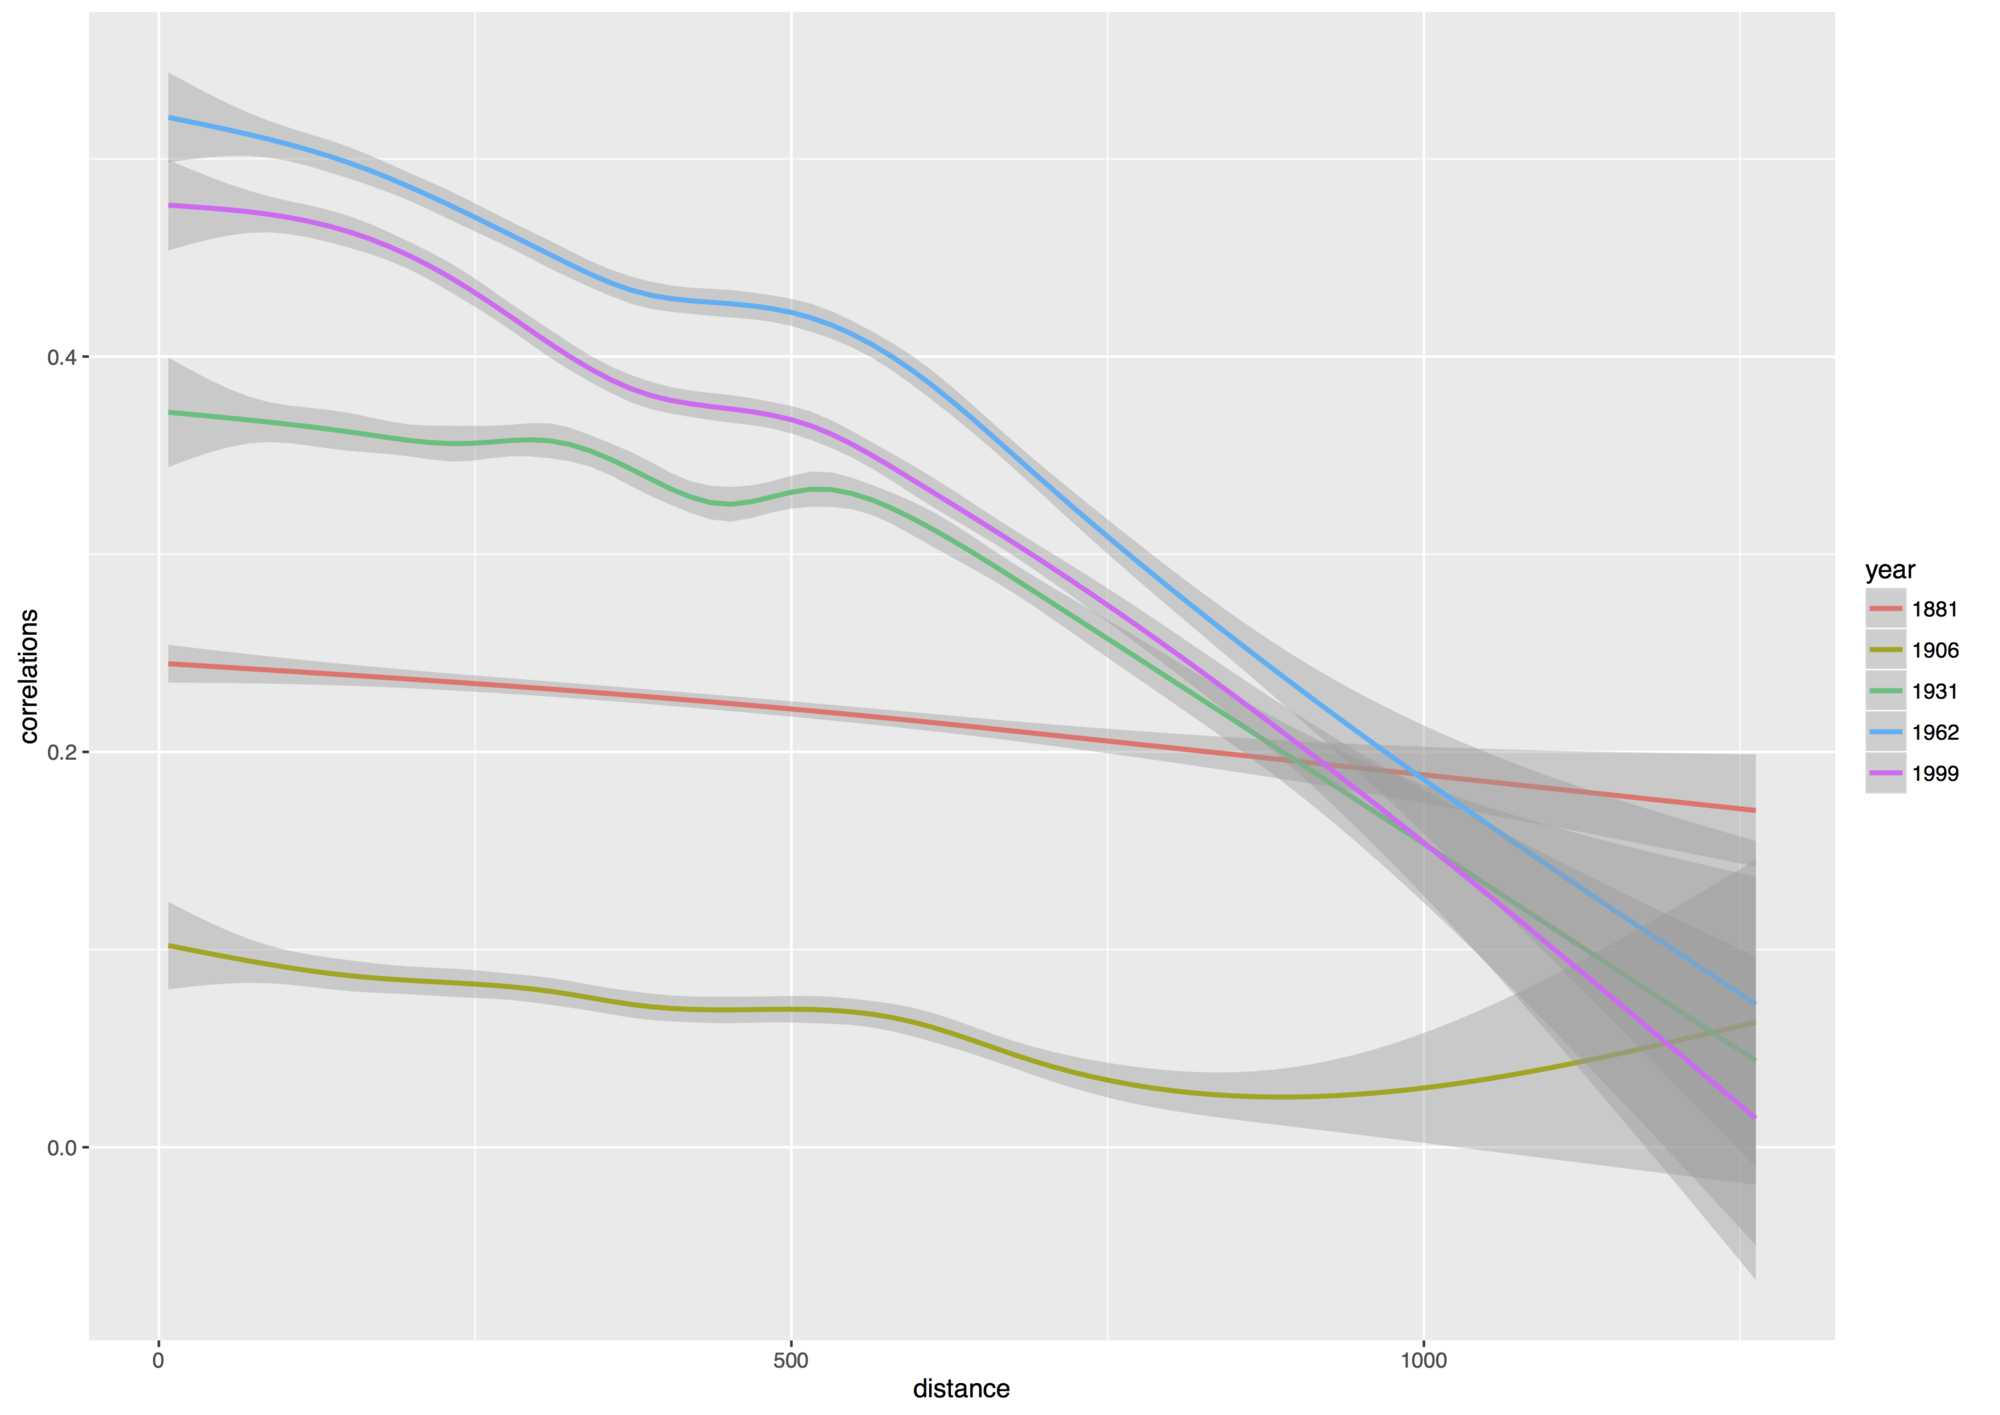
\includegraphics[width=\linewidth]{Figures/Final/4-3-2-fig-interactiongibrat-ts-correlations}
\caption[Time-series correlations][Corrélation de la croissance en fonction de la distance]{\textbf{Time-series correlations as a function of distance.} Solid line correspond to smoothed correlations, computed between each pairs of normalized log-returns of population time-series, on successive periods given by curve color.\label{fig:interactiongibrat:ts-correlations}}{\textbf{Corrélations entre séries temporelles en fonction de la distance.} Les lignes pleines correspondent aux corrélations lissées, calculées entre chaque paire des log-returns normalisés des séries temporelles de population, sur des périodes successives données par la couleur de la courbe.\label{fig:interactiongibrat:ts-correlations}}
\end{figure}
%%%%%%%%%%%%%%%%%%%%%%%%%





\paragraph{Model Exploration}{Exploration du modèle}


%\paragraph{Implementation}


\bpar{
Data preprocessing, result processing and models profiling are implemented in \texttt{R}. For performances reasons and an easier integration into the OpenMole software for model exploration~\citep{reuillon2013openmole}, a \texttt{scala} version was also developed. The question of trade-off between implementation performance and interoperability is a typical issue in this kind of model, as a fully blind exploration and calibration can be misleading for further research directions or thematic interpretations. A NetLogo implementation, allowing interactive exploration and dynamical visualization, was also developed for this reason. Source code for models, cleaned raw data, simulation data, and results used in this paper are available on the open repository of the project at \texttt{https://github.com/AnonymousAuthor1/InteractionGibrat.git}. We show in Figure~\ref{fig:interactiongibrat:interface} an example of model output. Cities color give city-level fit error and their size the population. Outliers can therefore easily be spotted (as Saint-Nazaire having the worst fit in the example shown) and possible regional effects identified. We illustrate in pink an example of geographical shortest path, from Rouen to Marseille, which reasonably corresponds to the actual current shortest path by highway. Top right plot shows trajectory in time for a given city, whereas the bottom right plot gives overall fit quality in time, by plotting simulated data against real data. The closest the curve is from the diagonal, the better the fit.
}{
La pré-traitement des données, le traitement des résultats et le profilage des modèles sont implémentés en \texttt{R}. Pour des raisons de performance et une intégration plus facile dans le logiciel OpenMole pour l'exploration de modèles~\cite{reuillon2013openmole}, une version \texttt{scala} a également été développée. La question du compromis entre performance d'implémentation et inter-opérabilité est un problème typique de ce genre de modèle, puisque des explorations et calibrations totalement aveugles peuvent être trompeuses pour les directions de recherches futures ou les interprétations thématiques. Une implémentation NetLogo, permettant l'exploration interactive et la visualisation dynamique, a également été développée pour cette raison. Le code source des modèles, les données brutes nettoyées, les données de simulation, et les résultats utilisés ici sont disponibles sur le dépôt ouvert du projet\footnote{A \url{https://github.com/JusteRaimbault/CityNetwork/tree/master/Models/NetworkNecessity/InteractionGibrat}. Les trois versions du modèle sont destinées à être reprises, réutilisées et étendues, et chaque implémentation a son utilité propre : la version \texttt{R} permet une intégration directe avec des scripts d'analyse de données, la version \texttt{scala} peut être utilisée comme plugin OpenMole, et la version NetLogo permet une exploration interactive et la visualisation directe des trajectoires.}. Nous montrons en Fig.~\ref{fig:interactiongibrat:interface} un exemple de sortie du modèle. Les couleurs des villes donnent l'écart à l'observation au niveau de la ville et leur taille la population. Les valeurs extrêmes peuvent ainsi être aisément repérées (comme Saint-Nazaire ayant le pire fit dans l'exemple montré) et des possibles effets régionaux identifiés. Nous illustrons en rose un exemple de plus court chemin géographique, de Rouen à Marseille, qui correspond raisonnablement au plus court chemin effectif actuel par autoroute. Le graphe du haut montre la trajectoire dans le temps pour une ville donnée, tandis que celui du bas donne la qualité globale de l'ajustement dans le temps, en traçant les données simulées en fonction des données réelles. Plus la courbe est proche de la diagonale, meilleur est l'ajustement.
}

%%%%%%%%%%%%%%%%%%%
\begin{figure}
%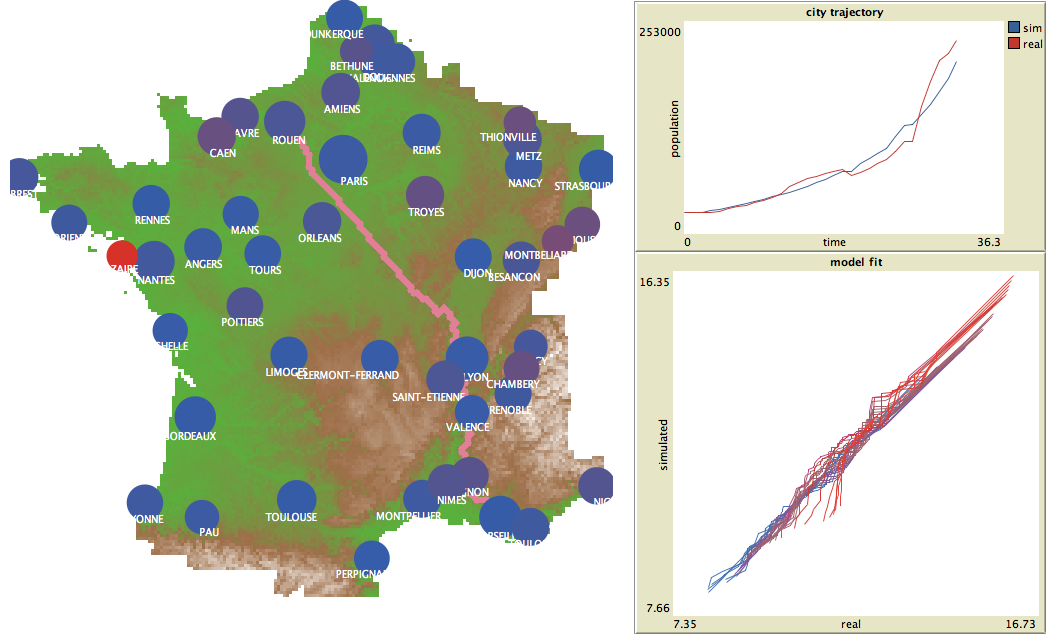
\includegraphics[width=\linewidth]{Figures/InteractionGibrat/Fig2}
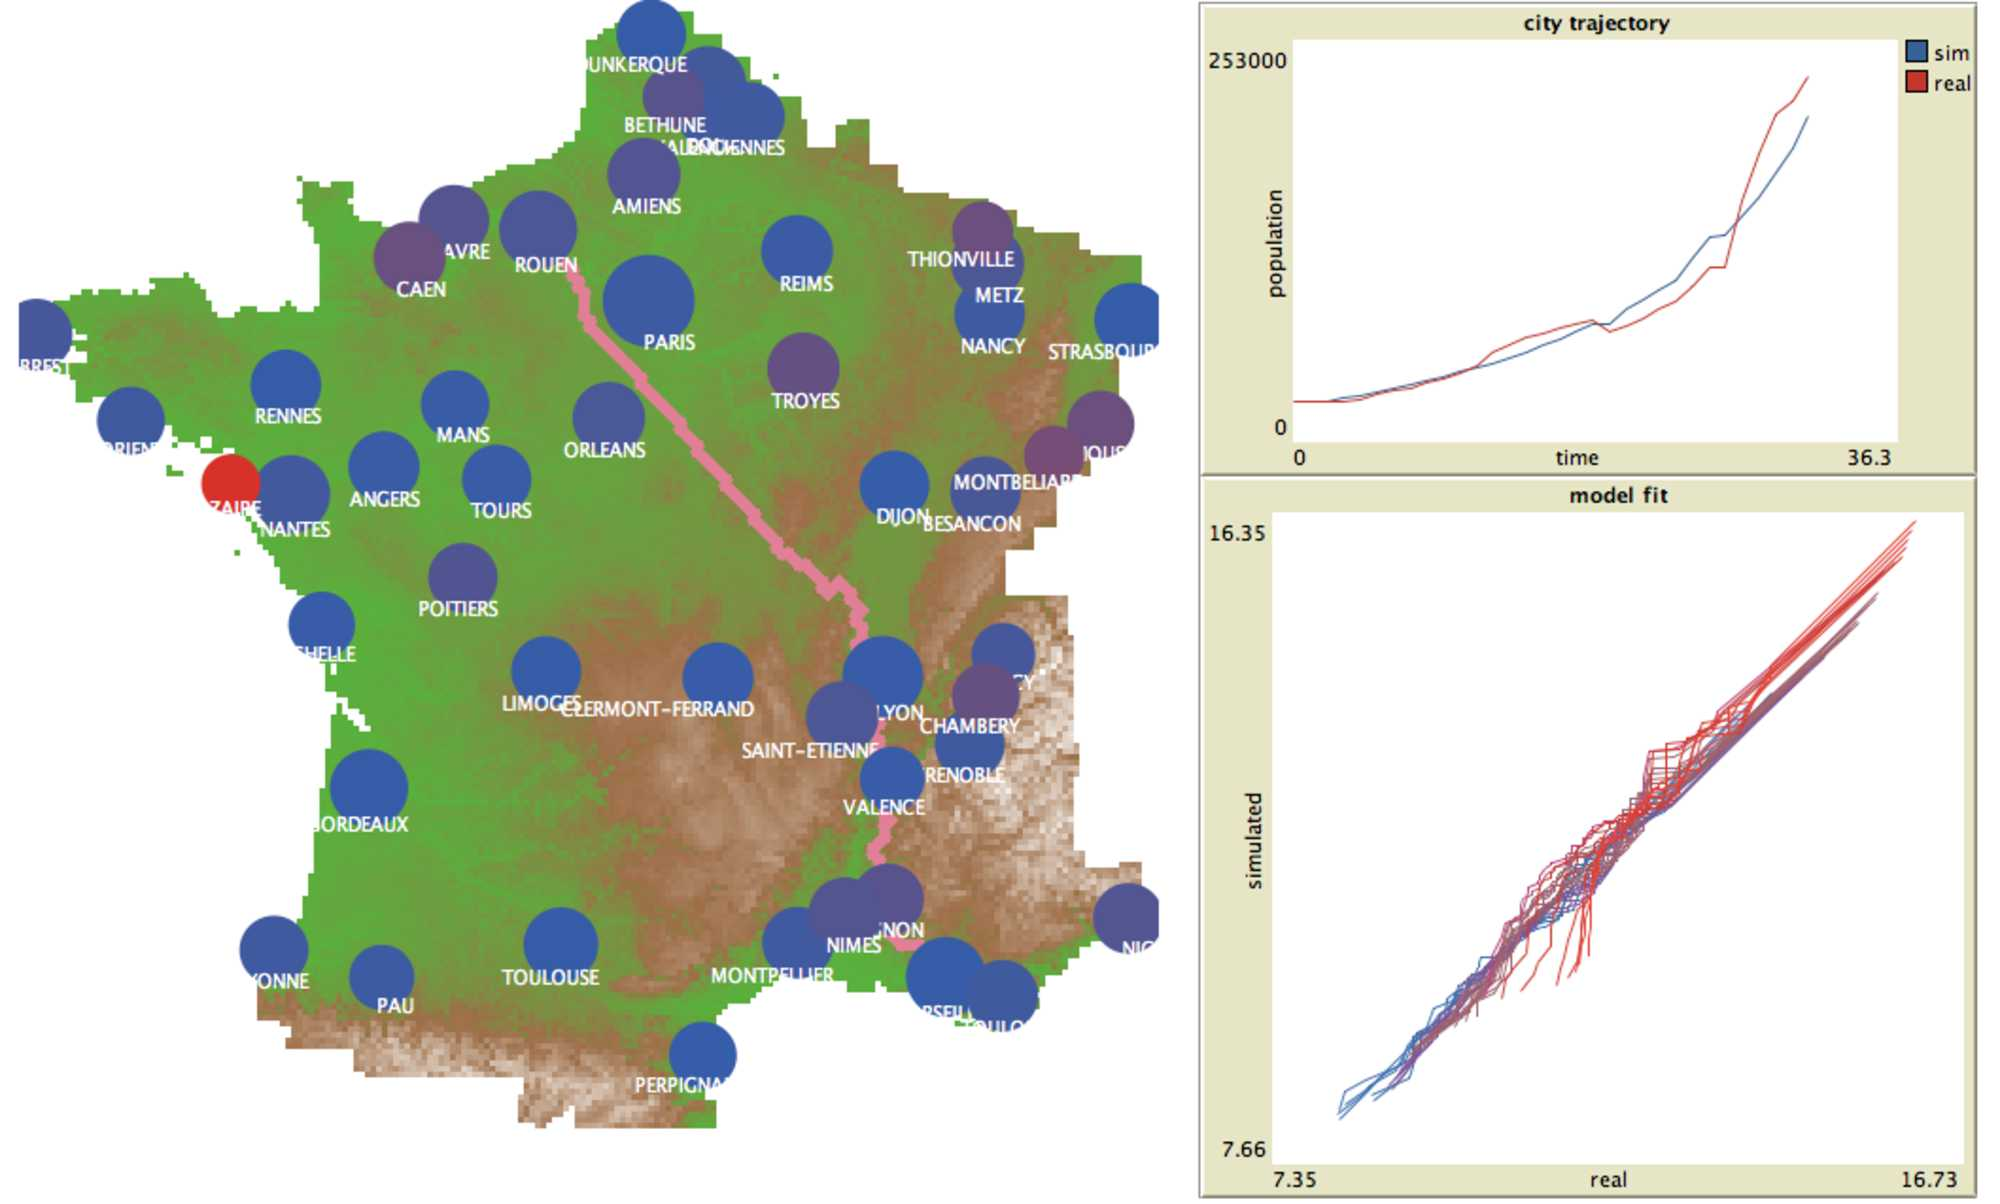
\includegraphics[width=\linewidth]{Figures/Final/4-3-2-fig-interactiongibrat-interface}
\caption[Model output][Interface du modèle d'interaction]{\textbf{Example of output of the model.} The graphical interface allows to explore interactively on which cities changes operate after a parameter change, what is necessary to interpret raw calibration results.\label{fig:interactiongibrat:interface}}{\textbf{Exemple de sortie du modèle.} L'interface graphique permet d'explorer de manière interactive sur quelles villes les changements s'opèrent après un changement de paramètres, ce qui est nécessaire pour interpréter les résultats bruts de calibration. La carte permet de visualiser les erreurs d'ajustement par ville (couleur) et leur population (taille). Nous illustrons en rose le plus court chemin géographique entre Rouen et Avignon. Le graphe supérieur permet de suivre dans le temps la trajectoire d'une ville donnée, en comparant la population simulée à la population réelle. Le graphe inférieur trace à chaque date l'ensemble des données simulées en fonction des données réelles : plus la courbe est proche de la diagonale plus l'ajustement est bon.\label{fig:interactiongibrat:interface}}
\end{figure}
%%%%%%%%%%%%%%%%%%%


%\paragraph{Behavior Patterns}

\bpar{
First model explorations, by simply sweeping fixed grids of the parameter space, already suggest the presence of network effects, in the sense that physical flow effectively have an influence on growth rates. We show in Figure~\ref{fig:interactiongibrat:networkeffects} a configuration of such a case. At fixed gravity parameters and growth rate, we study variations of the parameters $w_N, d_N$ and $\gamma_N$ and the corresponding response of $\varepsilon_G$ and $\varepsilon_L$. At fixed values of $\gamma_N$, we observe similar behaviors of the indicators when $w_N$ and $d_N$ change. The existence of a minimum of both as a function of $d_N$, that becomes stronger when $w_N$ increases, shows that introducing the network feedback terms improves local and global fits compared to the gravity model alone, i.e. that the associated process have potential explanatory power for growth patterns.
}{
Les premières explorations du modèle, en parcourant simplement des grilles fixées de l'espace des paramètres, suggèrent déjà la présence d'effets de réseau, au sens de flux physiques ayant effectivement une influence sur la reproduction des taux de croissance observés. Nous montrons en Fig.~\ref{fig:interactiongibrat:networkeffects} une configuration dans laquelle c'est le cas. À paramètres de gravité et taux de croissance fixés, nous étudions les variations des paramètres $w_N, d_N$ et $\gamma_N$ et la réponse correspondante de $\varepsilon_G$ et $\varepsilon_L$. A des valeurs fixes de $\gamma_N$, on observe un comportement similaire des indicateurs quand $w_N$ et $d_N$ varient. L'existence d'un minimum pour les deux comme fonction de $d_N$, qui devient plus marqué quand $w_N$ augmente, montre que l'introduction du terme de rétroaction du réseau améliore les fits locaux et globaux en comparaison du modèle de gravité seul, i.e. que les processus associés ont un pouvoir explicatif pour les motifs de croissance.
}


%%%%%%%%%%%%%%%%%%%%
\begin{figure}
%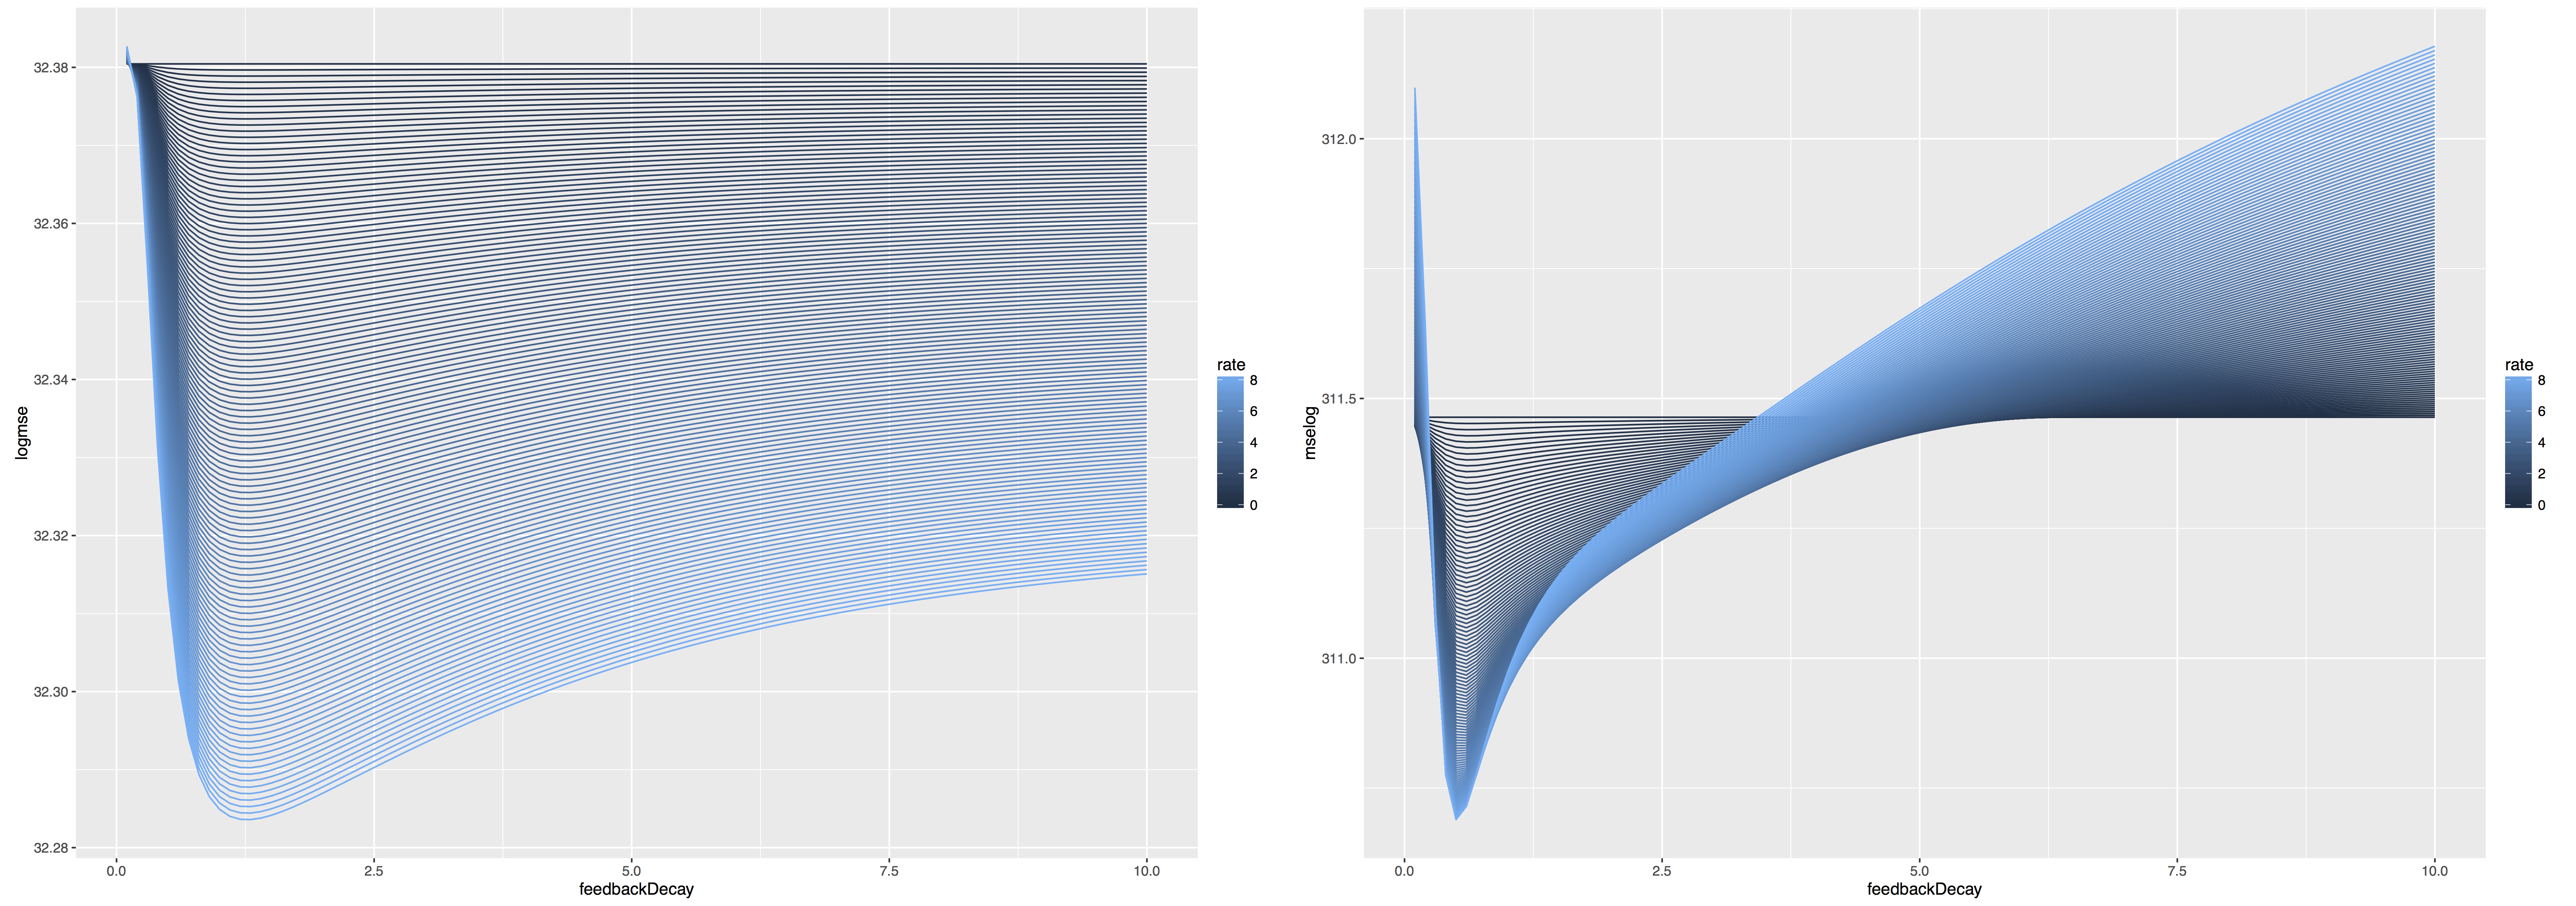
\includegraphics[width=\linewidth]{Figures/InteractionGibrat/Fig3}
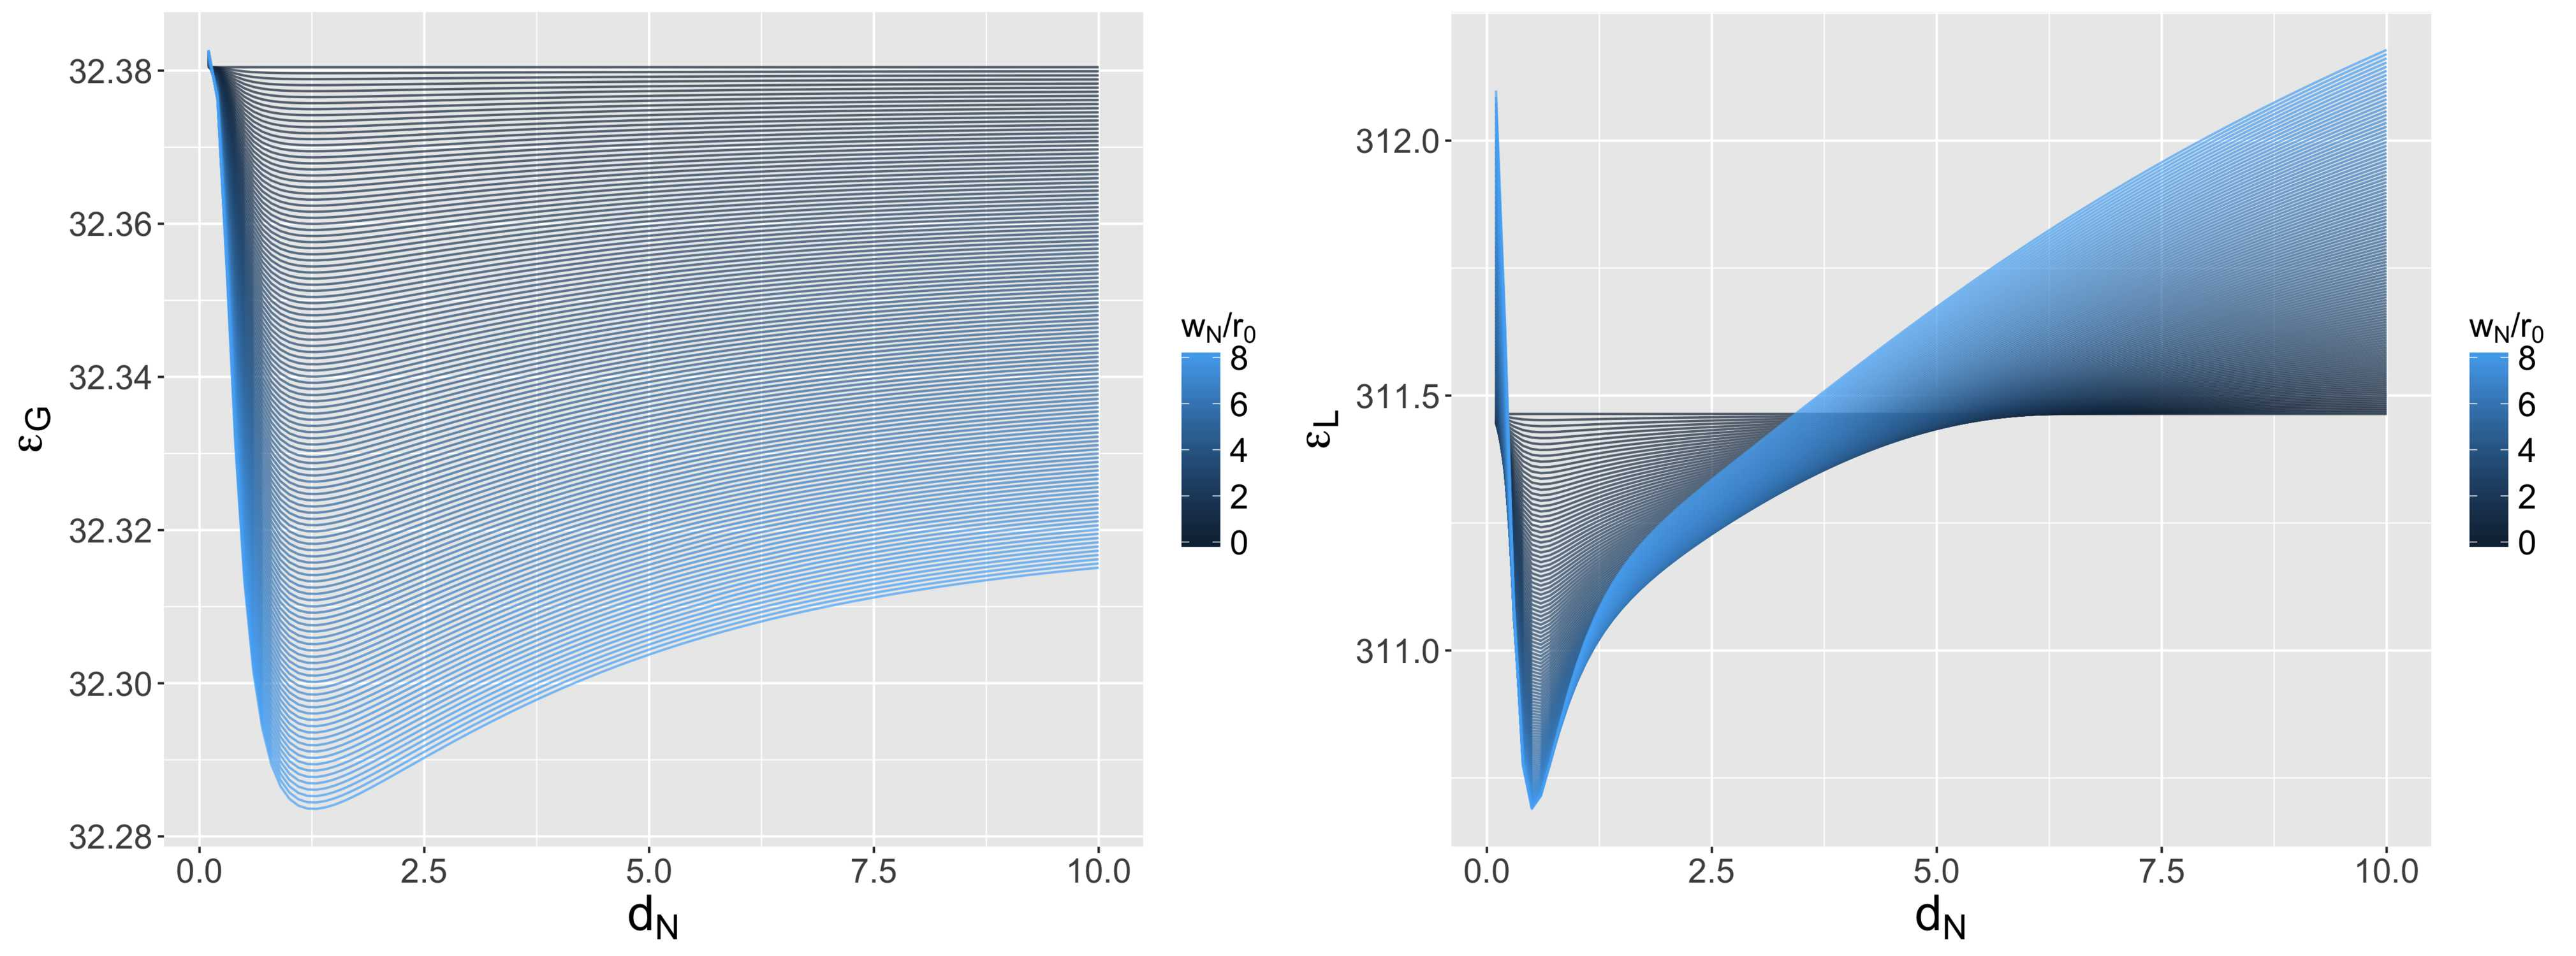
\includegraphics[width=\linewidth]{Figures/Final/4-3-2-fig-interactiongibrat-networkeffects}
\caption[Evidence of network effects][Révélation d'effets de réseau]{\textbf{Evidence of network effects revealed by model exploration.} Left plot gives $\varepsilon_G$ as a function of $d_N$ for varying $r_0/w_N$, at fixed gravity effect and $\gamma_N=3$. Right plot is similar for $\varepsilon_L$.\label{fig:interactiongibrat:networkeffects}}{\textbf{Effets de réseau révélés par l'exploration du modèle.} Le graphe de gauche donne $\varepsilon_G$ comme fonction de $d_N$ pour $w_N/r_0$ variant (\texttt{rate}), à effet de gravité fixe et $\gamma_N=3$. Le graphe de droite est similaire pour $\varepsilon_L$. Partant d'un modèle gravitaire pur (courbe horizontale pour $w_N$), la prise en compte progressive du réseau augmente les performances au regard des deux objectifs, dans une plage restreinte pour $d_N$. Les valeurs de $d_N$ donnant les minima correspondent à la distance typique de l'effet du réseau.\label{fig:interactiongibrat:networkeffects}}
\end{figure}
%%%%%%%%%%%%%%%%%%%%






\paragraph{Calibrating the Gravity Model}{Calibration du modèle de gravité}


%%%%%%%%%%%%%%%%%%%%
\begin{figure}
%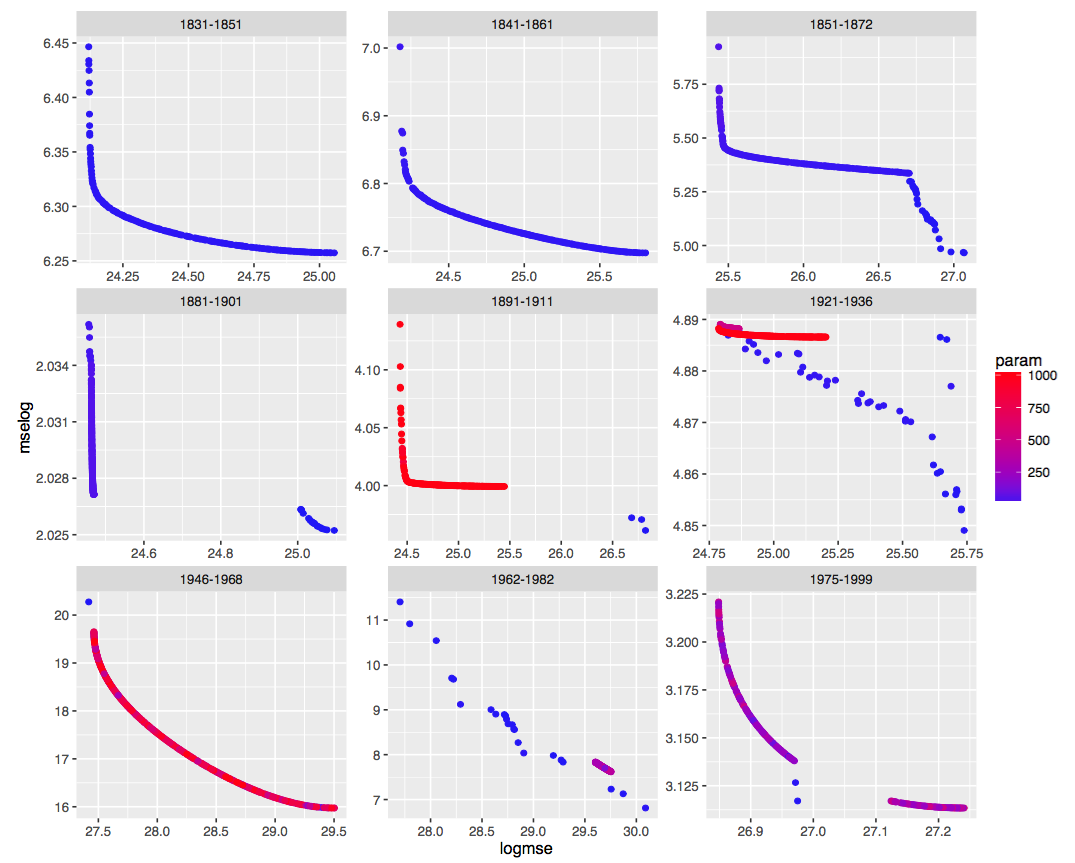
\includegraphics[width=\linewidth]{Figures/InteractionGibrat/Fig4}
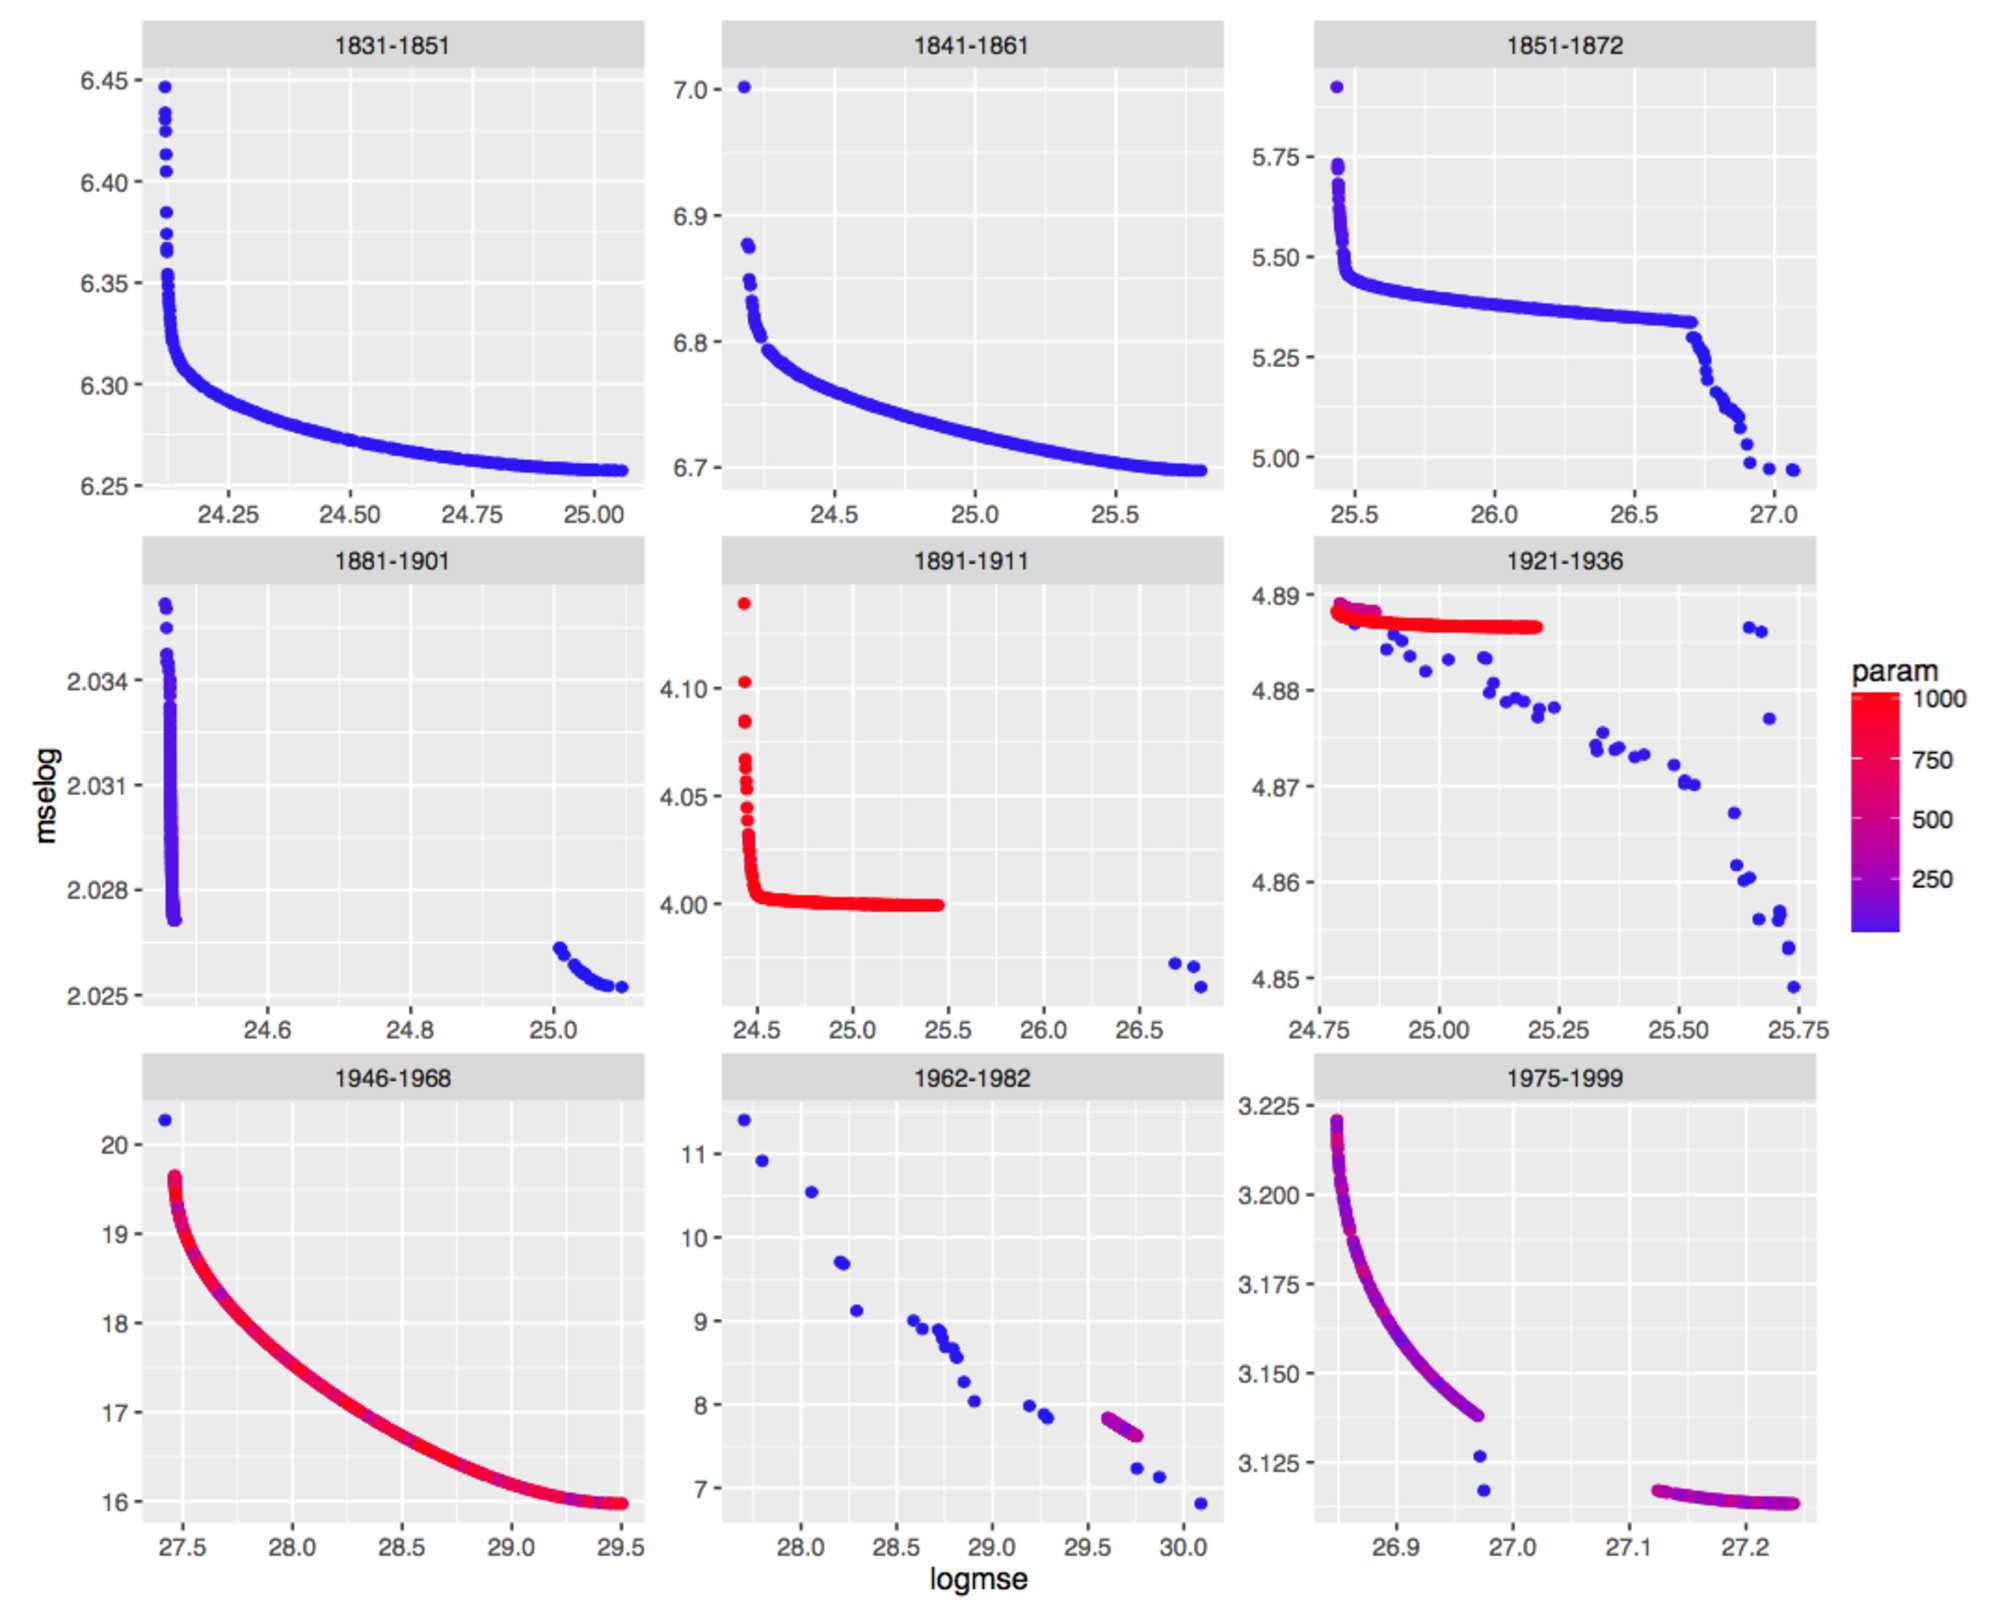
\includegraphics[width=\linewidth]{Figures/Final/4-3-2-fig-interactiongibrat-gravity-pareto}
\caption[Calibrating the Gravity Model][Calibration du modèle de gravité]{\textbf{Calibrating the Gravity Model.} Pareto-front on successive periods. Color level gives the value of distance decay parameter.\label{fig:interactiongibrat:gravity-pareto}}{\textbf{Calibration du modèle de gravité.} Fronts de Pareto sur les périodes successives. La couleur donne la valeur du paramètre de décroissance de la distance.\label{fig:interactiongibrat:gravity-pareto}}
\end{figure}
%%%%%%%%%%%%%%%%%%%%


%%%%%%%%%%%%%%%%%%%%
\begin{figure}
%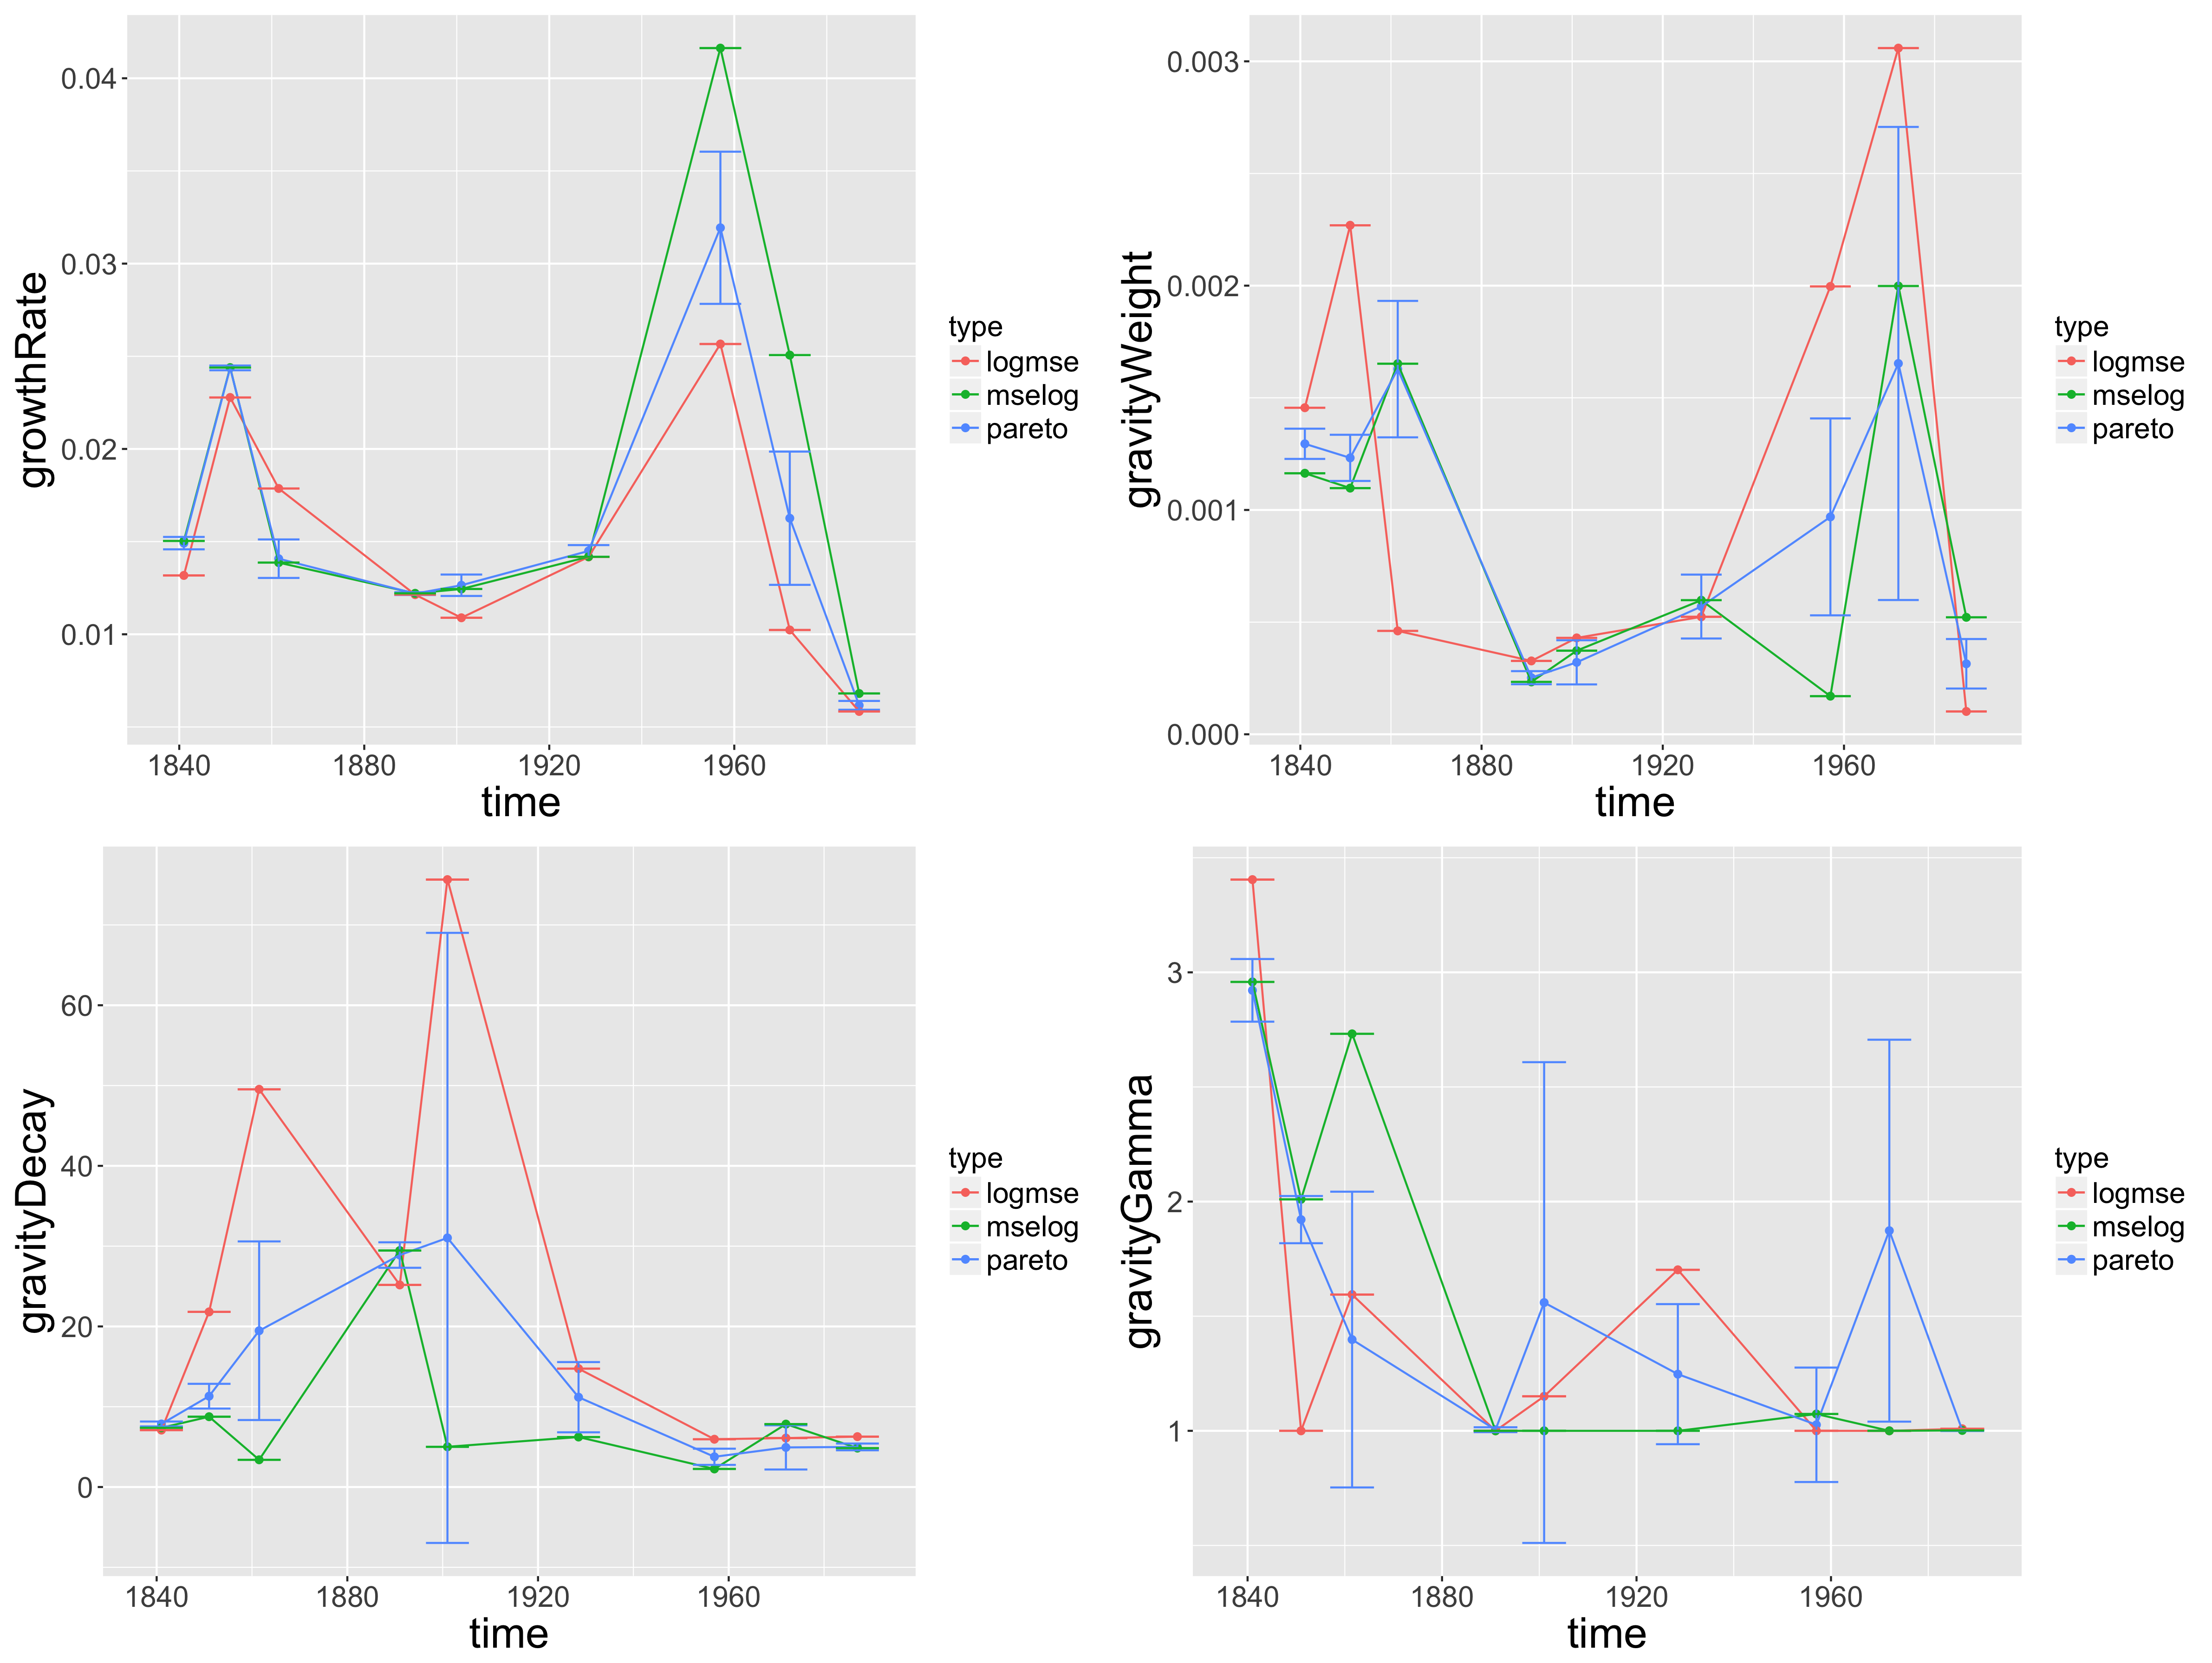
\includegraphics[width=\linewidth]{Figures/InteractionGibrat/Fig5}
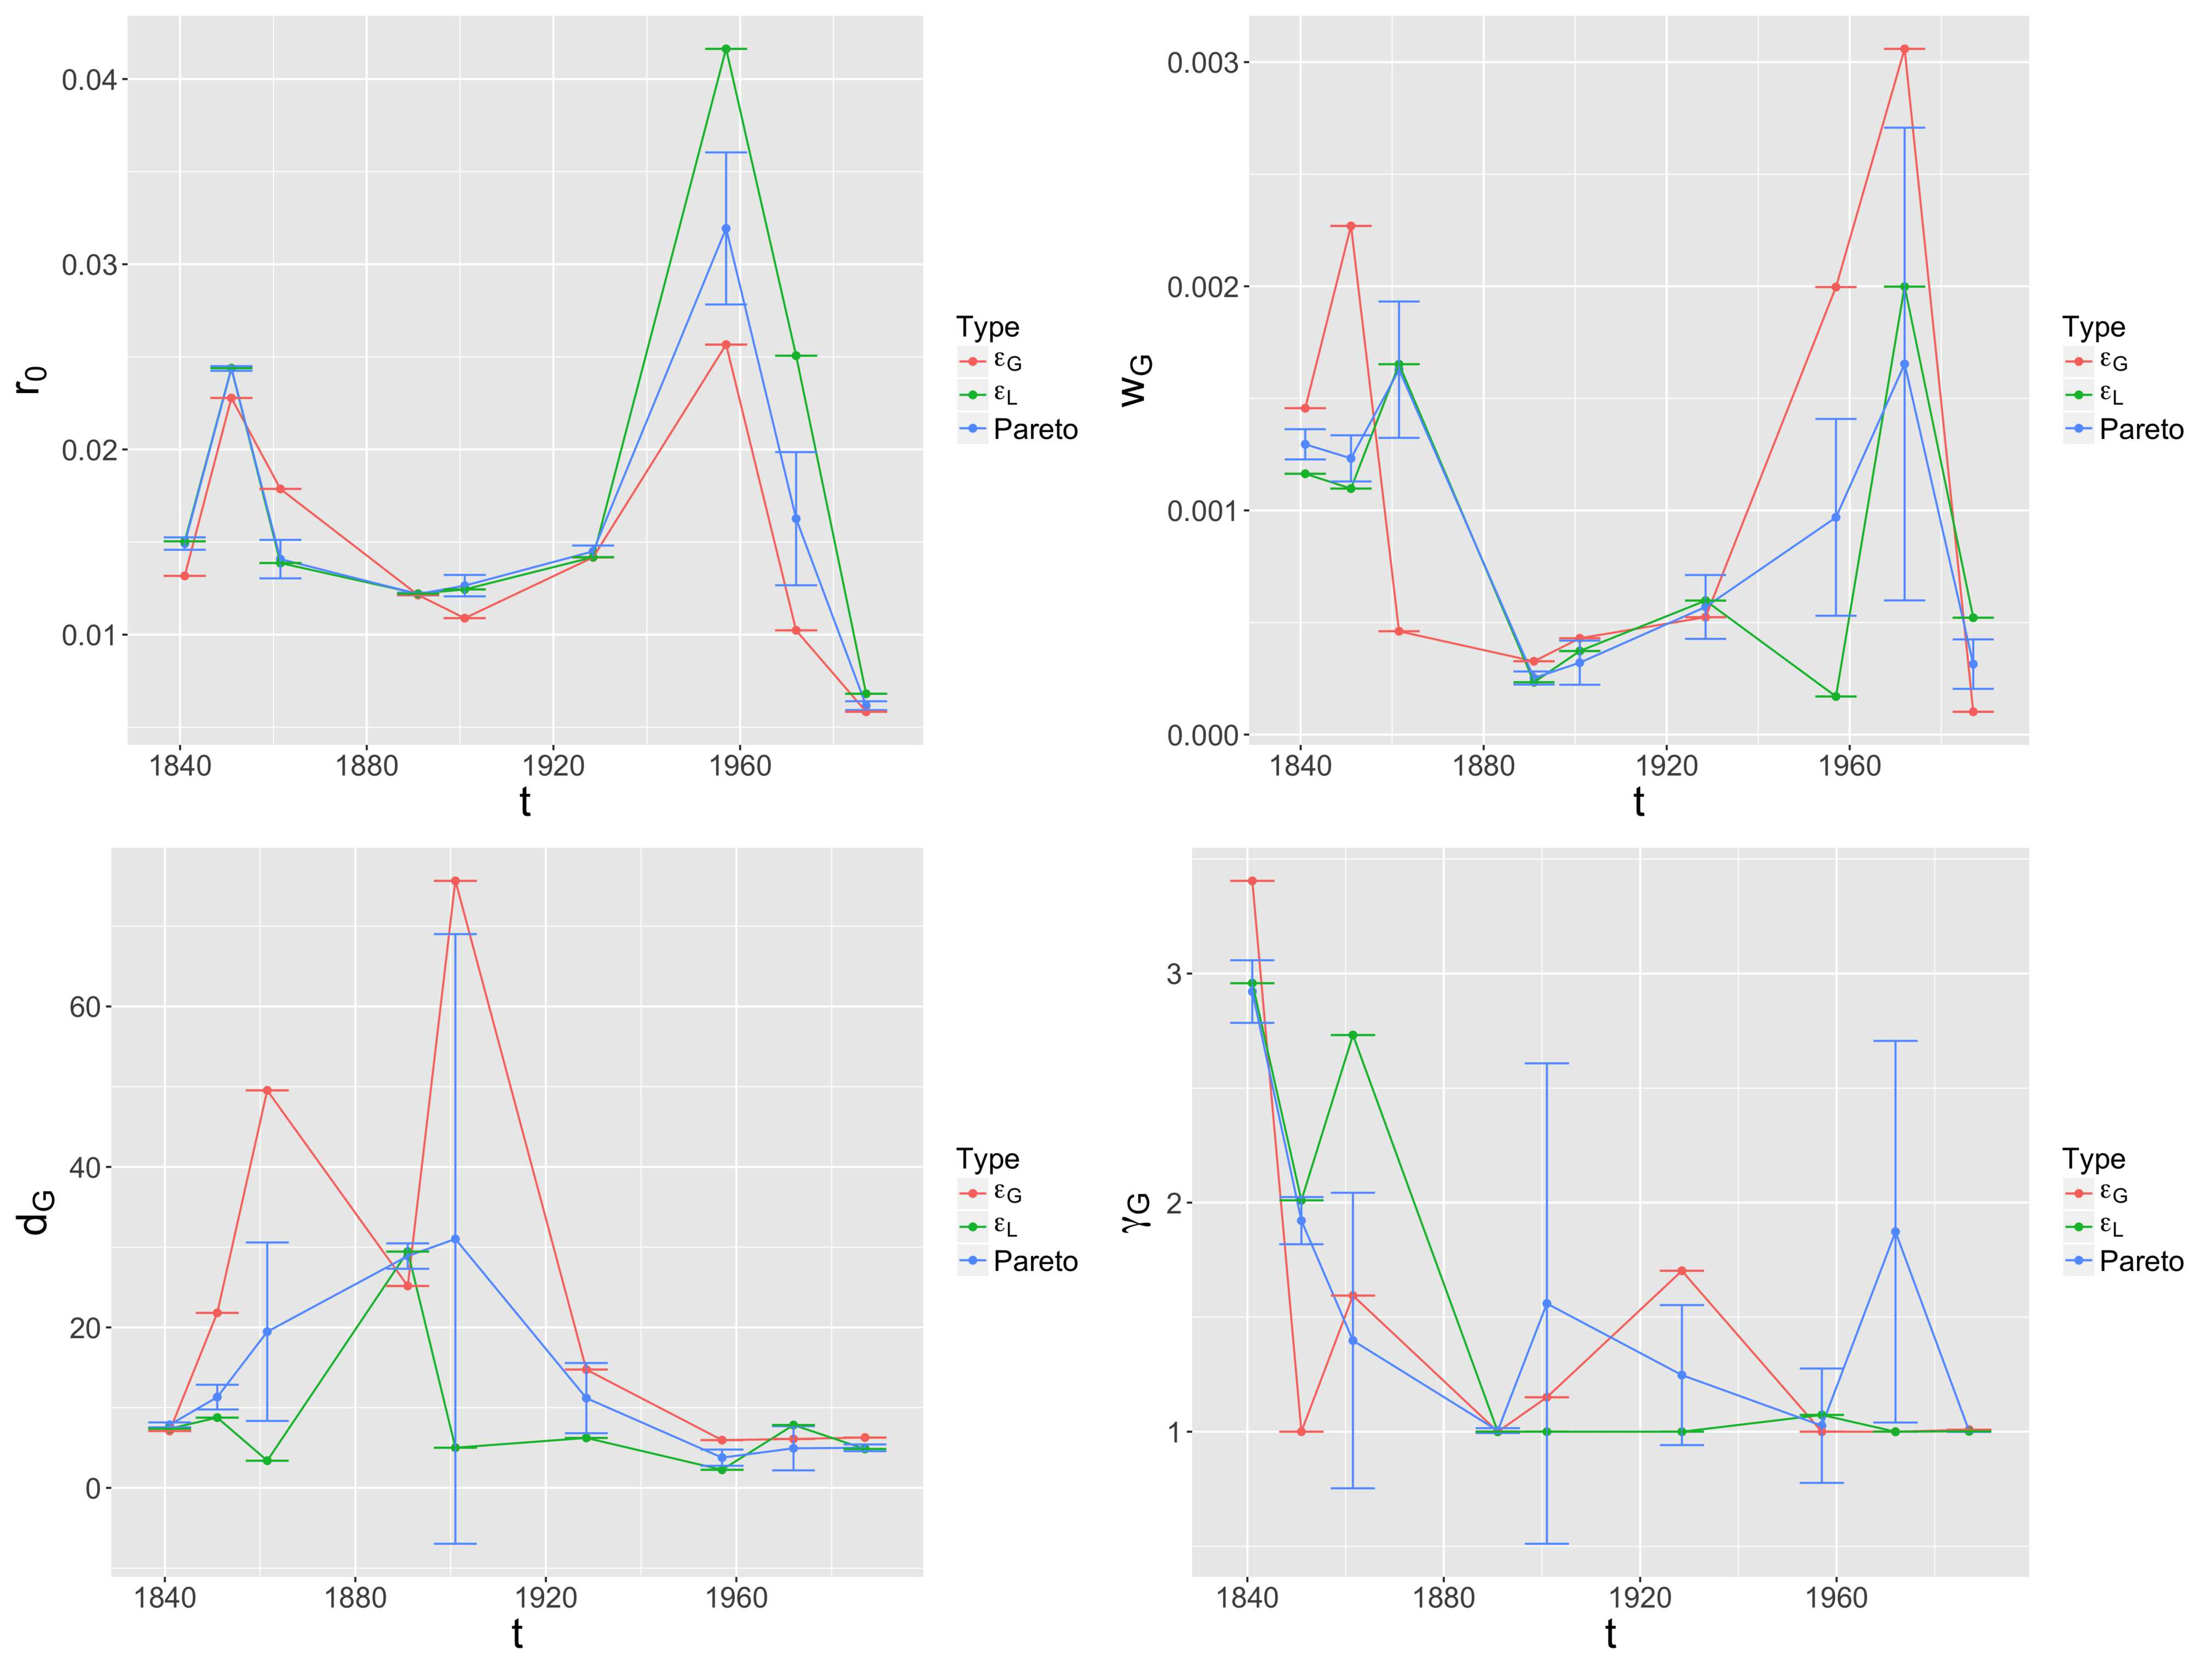
\includegraphics[width=\linewidth]{Figures/Final/4-3-2-fig-interactiongibrat-gravity-params}
\caption[Calibrated parameters][Valeurs des paramètres calibrés]{\textbf{Calibrated parameters for gravity model only.} Each plot gives fitted values in time for each parameter. Red and Green curves correspond to best points for $\varepsilon_G$ (respectively $\varepsilon_L$), whereas the blue curves give the average value over the Pareto front with standard deviation.\label{fig:interactiongibrat:gravity-params}}{\textbf{Valeurs des paramètres calibrés pour le modèle de gravité seul.} Chaque graphe donne les valeur ajustées dans le temps pour chaque paramètre. Les courbes rouge et verte correspondent aux points optimaux pour $\varepsilon_G$ (respectivement $\varepsilon_L$), tandis que la courbe bleue donne la valeur moyenne sur l'ensemble du front de Pareto avec la déviation standard. Selon qu'on s'intéresse à la performance sur les petites villes (\texttt{mselog}), les grandes villes (\texttt{logmse}) ou des compromis (\texttt{pareto}), on obtiendra une évolution des paramètres pouvant différer. Des grandes tendances se dégagent, comme le double pic du taux de croissance endogène (\texttt{growthRate}) qui se retrouve dans le poids des interactions, et une hiérarchie décroissante des interactions.\label{fig:interactiongibrat:gravity-params}}
\end{figure}
%%%%%%%%%%%%%%%%%%%%


\bpar{
We now use the model to indirectly extract information on processes in time. Indeed under assumption of non-stationarity, temporal evolution of locally fitted parameters show the evolution of the corresponding aspect of the processes. In a first experiment, we set $w_N=0$ and calibrate the model with four parameters on the 9 successive 20 years time windows. The optimization problem associated to model calibration does not present features allowing an easy solving (closed-form of a likelihood function, convexity or sparsity of the optimization problem), we must rely on alternative techniques to solve it. Brute force grid search is rapidly limited by the dimensionality curse. Classical methods~\citep{batty1972calibration} such as gradient descent fail because of the rather complicated shape of the optimisation landscape. Calibration using Genetic Algorithms (GA) are an efficient solution to find approximate solutions in a reasonable time. OpenMole embeds a collection of such meta-heuristics for different purposes: \cite{schmitt2014half} demonstrates the capabilities of these methods to calibrate models of simulation. In our case, it furthermore allow to do a bi-objective calibration on $(\varepsilon_G,\varepsilon_L)$. We use the standard steady state GA provided by OpenMole, distributed on 25 islands, with population of 200 and 100 generations.
}{
Nous utilisons à présent le modèle pour extraire de l'information de manière indirecte sur les processus dans le temps. En effet sous l'hypothèse de non-stationnarité, l'évolution temporelle des paramètres ajustés localement montre l'évolution de l'aspect des processus correspondant. Dans une première expérience, nous fixons $w_N=0$ et calibrons le modèle avec quatre paramètres sur les neuf périodes temporelles successives de 20 ans. Le problème d'optimisation associé à la calibration du modèle ne présente pas de caractéristiques le rendant agréable à résoudre (expression fermée d'une fonction de likelihood, convexité ou caractère creux du problème d'optimisation), nous devons nous reposer sur des techniques alternatives pour le résoudre. Une exploration de grille par force brute est rapidement limitée par le sort de la dimension. Les méthodes classiques~\cite{batty1972calibration} comme une descente du gradient échouent à cause de la forme assez compliquée du paysage d'optimisation. La calibration par Algorithme Génétique (GA) est une solution efficace pour trouver des solutions approximatives en un temps raisonnable. OpenMole inclut une collection de telles méta-heuristiques pour différents buts : \cite{schmitt2014half} démontre les potentialités de ces méthodes pour calibrer les modèles de simulation. Dans notre cas, cela permet de plus de procéder à une optimisation bi-objectif sur $(\varepsilon_G,\varepsilon_L)$. Nous utilisons le GA steady state standard fournit par OpenMole, distribué sur 25 îles, avec une population de 200 individus et 100 générations\footnote{Voir~\cite{pumain2017urban} pour la présentation la plus récente des méthodes de calibration de modèles urbains par algorithme génétique fournit par OpenMole.}.
}


\bpar{
We show in Figure~\ref{fig:interactiongibrat:gravity-pareto} the calibration results on successive periods, by plotting final population in the indicator space. As expected, Pareto fronts that corresponds to compromises between the two opposite objectives are the rule. It means that the model cannot be accurate both globally and locally, and an intermediate solution has to be found. This may due to the fact that interaction range changes with city size (i.e. that terms in the potential are no longer separable), that we keep as a possible model development. The shape of the Pareto front are revealing the chaotic optimisation landscape, as for some periods such as 1921-1936 or 1962-1982 fronts are not regular and sparse. The change in shapes also translates different dynamical regimes across the periods: for 1881-1901, the quasi-vertical shape followed by an isolated front at high $\varepsilon_G$ values reveals a quasi-binary model behavior in the optimal regimes, in the sense that improving $\varepsilon_L$ under the limit is only possible through a qualitative jump at a high price for $\varepsilon_G$.
}{
Nous montrons en Fig.~\ref{fig:interactiongibrat:gravity-pareto} les résultats de la calibration sur les périodes successives, en représentant la population finale dans l'espace des indicateurs. Comme attendu, des fronts de Pareto correspondant à des compromis entre les deux objectifs opposés sont la règle. Cela signifie que le modèle ne peut pas être précis à la fois globalement et localement, et qu'une solution intermédiaire doit être trouvée. Cela peut être dû au fait que la portée d'interaction change avec la taille de la ville (i.e. que les termes dans le potentiel ne sont plus séparables), que nous gardons comme un développement potentiel du modèle. La forme des fronts de Pareto révèle un paysage d'optimisation chaotique, puisque pour certaines périodes comme 1921-1936 ou 1962-1982 les fronts ne sont pas réguliers et éparpillés. Le changement dans les formes traduit également différents régimes dynamiques selon les périodes : pour 1881-1901, la forme quasi-verticale suivi par un front isolé à de fortes valeurs de $\varepsilon_G$ révèle un comportement quasi-binaire du modèle dans les régimes optimaux, au sens où améliorer $\varepsilon_L$ sous la limite n'est possible uniquement à travers un saut qualitatif à un fort coût pour $\varepsilon_G$.
}


\bpar{
The values taken by $d_G$ for periods 1892-1911 and 1921-1936 show that larger cities have longer interaction range, as high value give better values of $\varepsilon_G$. We show in Figure~\ref{fig:interactiongibrat:gravity-params} the values of fitted parameters in time, averaged over the Pareto front and for best single-objective solutions. First, the two peaks patterns for $r_0$ corresponds roughly to the patterns observed in average growth rates. The evolution of $w_G$ has a similar shape but lagged by 20 years: it can be interpreted as a repercussion of endogenous growth on interaction patterns in the following years, which is consistent with an interpretation of the interaction process in terms of migration. The values of $d_G$, with an increase until 1900 followed by a progressive decrease, is consistent with the behavior of empirical correlations commented above: the first 50 years windows have higher interaction range what corresponds to flat correlation curves. Finally, the level of hierarchy $\gamma_G$ has regularly decreased, corresponding to an attenuation of the power of large cities that can be understood in terms of progressive decentralization in France that has been fostered by the administration.
}{
Les valeurs prises par $d_G$ pour les périodes 1892-1911 et 1921-1936 montrent que les grandes villes ont des portées d'interaction plus grandes, puisqu'une valeur plus grande donne des meilleurs valeurs pour $\varepsilon_G$. Nous montrons en Fig.~\ref{fig:interactiongibrat:gravity-params} les valeurs des paramètres ajustés dans le temps, par leur moyenne sur le front de Pareto et pour les deux meilleurs solutions à objectif simple. Tout d'abord, les deux motifs en pic pour $r_0$ correspondent globalement au comportement observé sur les taux de croissance moyens. L'évolution de $w_G$ a une forme similaire mais décalée de 20 ans : cela peut être interprété comme une répercussion de la croissance endogène sur les motifs d'interaction les années suivantes, ce qui est cohérent avec une interprétation des processus d'interaction en termes de migration. Les valeurs de $d_G$, avec une augmentation jusqu'en 1900 suivie d'une décroissance progressive, est cohérent avec le comportement des corrélations empiriques commenté précédemment : les deux premières fenêtres de 50 ans ont des portées d'interaction plus grandes ce qui correspond à des courbes de corrélations plates. Enfin, le niveau de hiérarchie $\gamma_G$ a été régulièrement décroissant, ce qu'on peut lire comme une atténuation du pouvoir des grandes villes, qui peut être comprise en termes de la décentralisation progressive en France qui a été encouragée par l'administration\footnote{Sachant que la réalité est forcément plus complexe et qu'une telle tendance peut être tirée aussi par une inscription plus globale dans un changement de nature des structures urbaines, dont témoigne par exemple l'émergence des MCR (voir~\ref{sec:casestudies}).}.
}



\paragraph{Unveiling Network Effects}{Effets de Réseau}


\bpar{
We now turn to the calibration of the full model on successive periods, in order to interpret parameters linked to network flows and gain insight into network effects. The full calibration is done in a similar way with seven parameters being free. We plot in Figure~\ref{fig:interactiongibrat:feedback} the fitted values in time for some of these parameters. The behavior of growth rate and of the gravity weight relative to growth rate, that is similar to the gravity model only, confirms that network effects are well at the second order and that endogenous growth and direct interactions are main driver. Network effects are however not negligible, as they improve the fit as shown before in model exploration, capturing therein second order processes. The evolution of $d_N$, corresponding to the range on which network influences the territories it goes through, shows a minimum in 1921-1936 to stabilize again later, but at a value lower that past values. This could correspond to the ``tunnel effect'', when high-speed transportation do not stop much. Indeed, the evolution of railway has witnessed a high decrease in local lines at a date similar to the minimum, and later the emergence of specific High Speed lines, explaining this lower final value. Hierarchy of flows have slightly decreased as for gravity, but are extremely high. This means that only flows between larger cities have a significant effect. This way, the model gives indirect information on the processes linked to network effects.
}{
Nous nous intéressons à présent à la calibration du modèle complet sur des périodes successives, dans le but d'interpréter les paramètres liés aux flux de réseau et obtenir des informations sur les effets de réseau. La calibration complète est faite de manière similaire avec les sept paramètres libres. Nous montrons en Fig.~\ref{fig:interactiongibrat:feedback} les values ajustées dans le temps pour certains de ces paramètres. Le comportement du taux de croissance et du poids de la gravité relatif au taux de croissance, qui est similaire au modèle de gravité seul, confirme que les effets de réseau sont bien au second ordre et que la croissance endogène et les interactions directes sont les facteurs principaux. Les effets de réseaux sont cependant loin d'être négligeables, puisqu'ils améliorent l'ajustement comme montré précédemment lors de l'exploration du modèle, capturant ainsi des processus de second ordre. L'évolution de $d_N$, correspondant à la portée sur laquelle le réseau influence le territoire qu'il traverse, montre un minimum en 1921-1936 pour se stabiliser à nouveau plus tard, mais à une valeur plus basse que les valeurs du passé. Cela pourrait correspondre à l'effet tunnel, puisque les transports à grande vitesse ne s'arrêtent peu sur les territoires qu'ils traversent. En effet, l'évolution du réseau ferré a témoigné une forte décroissance des lignes locales à une date similaire au minimum, et plus tard l'émergence de lignes à grande vitesse spécifiques, ce qui expliquerait cette valeur finale plus basse. La hiérarchie des flux a été légèrement décroissante comme pour la gravité, mais est extrêmement haute. Cela signifie que seuls les flux entre les grandes villes ont un effet significatif. Ainsi, le modèle donne une information indirecte sur les processus liés aux effets de réseau.
}

% \comment[FL]{c'est interessant et vraiment dans le coeur de ta these}

Nous retenons de la calibration du modèle complet les faits stylisés suivants :
\begin{itemize}
	\item Des effets des réseaux sont capturés au second ordre par le modèle.
	\item Les variations de la portée de l'effet du réseau suggèrent l'émergence de l'effet tunnel.
	\item Les flux principaux dominent largement dans l'effet de réseau.
\end{itemize}



%%%%%%%%%%%%%%%%%%%%%%%%%%%
\begin{figure}
%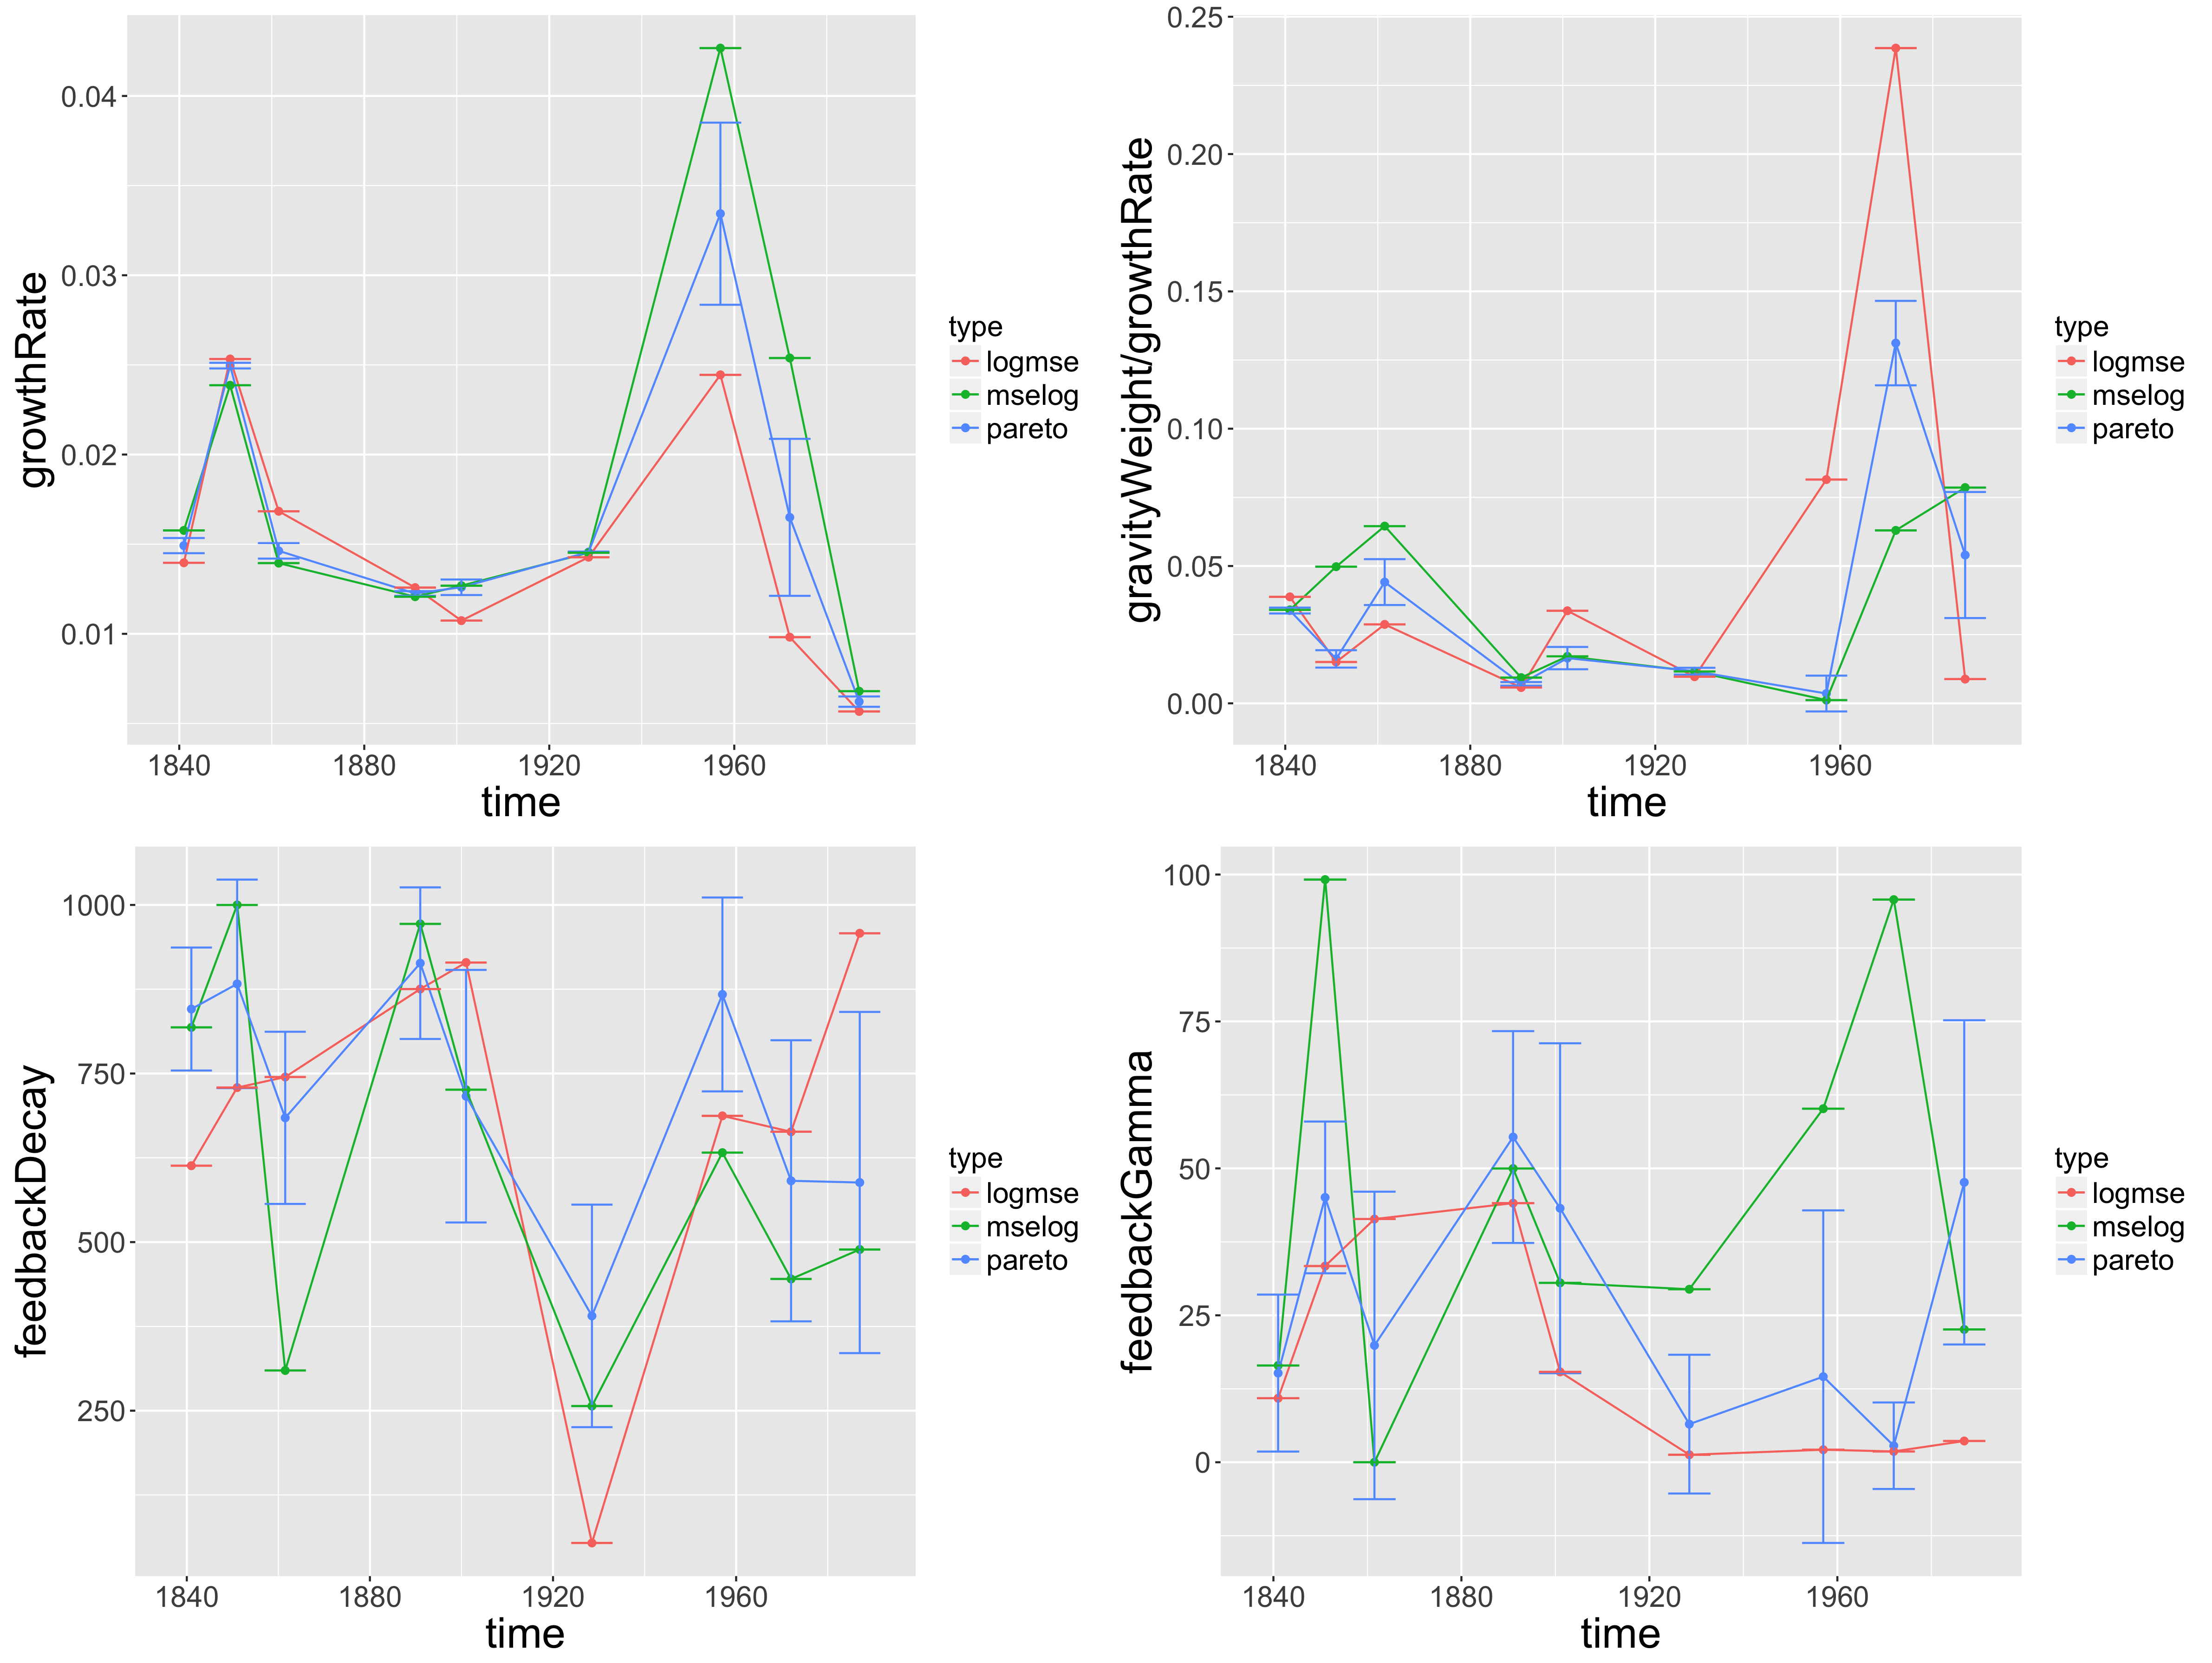
\includegraphics[width=\linewidth]{Figures/InteractionGibrat/Fig6}
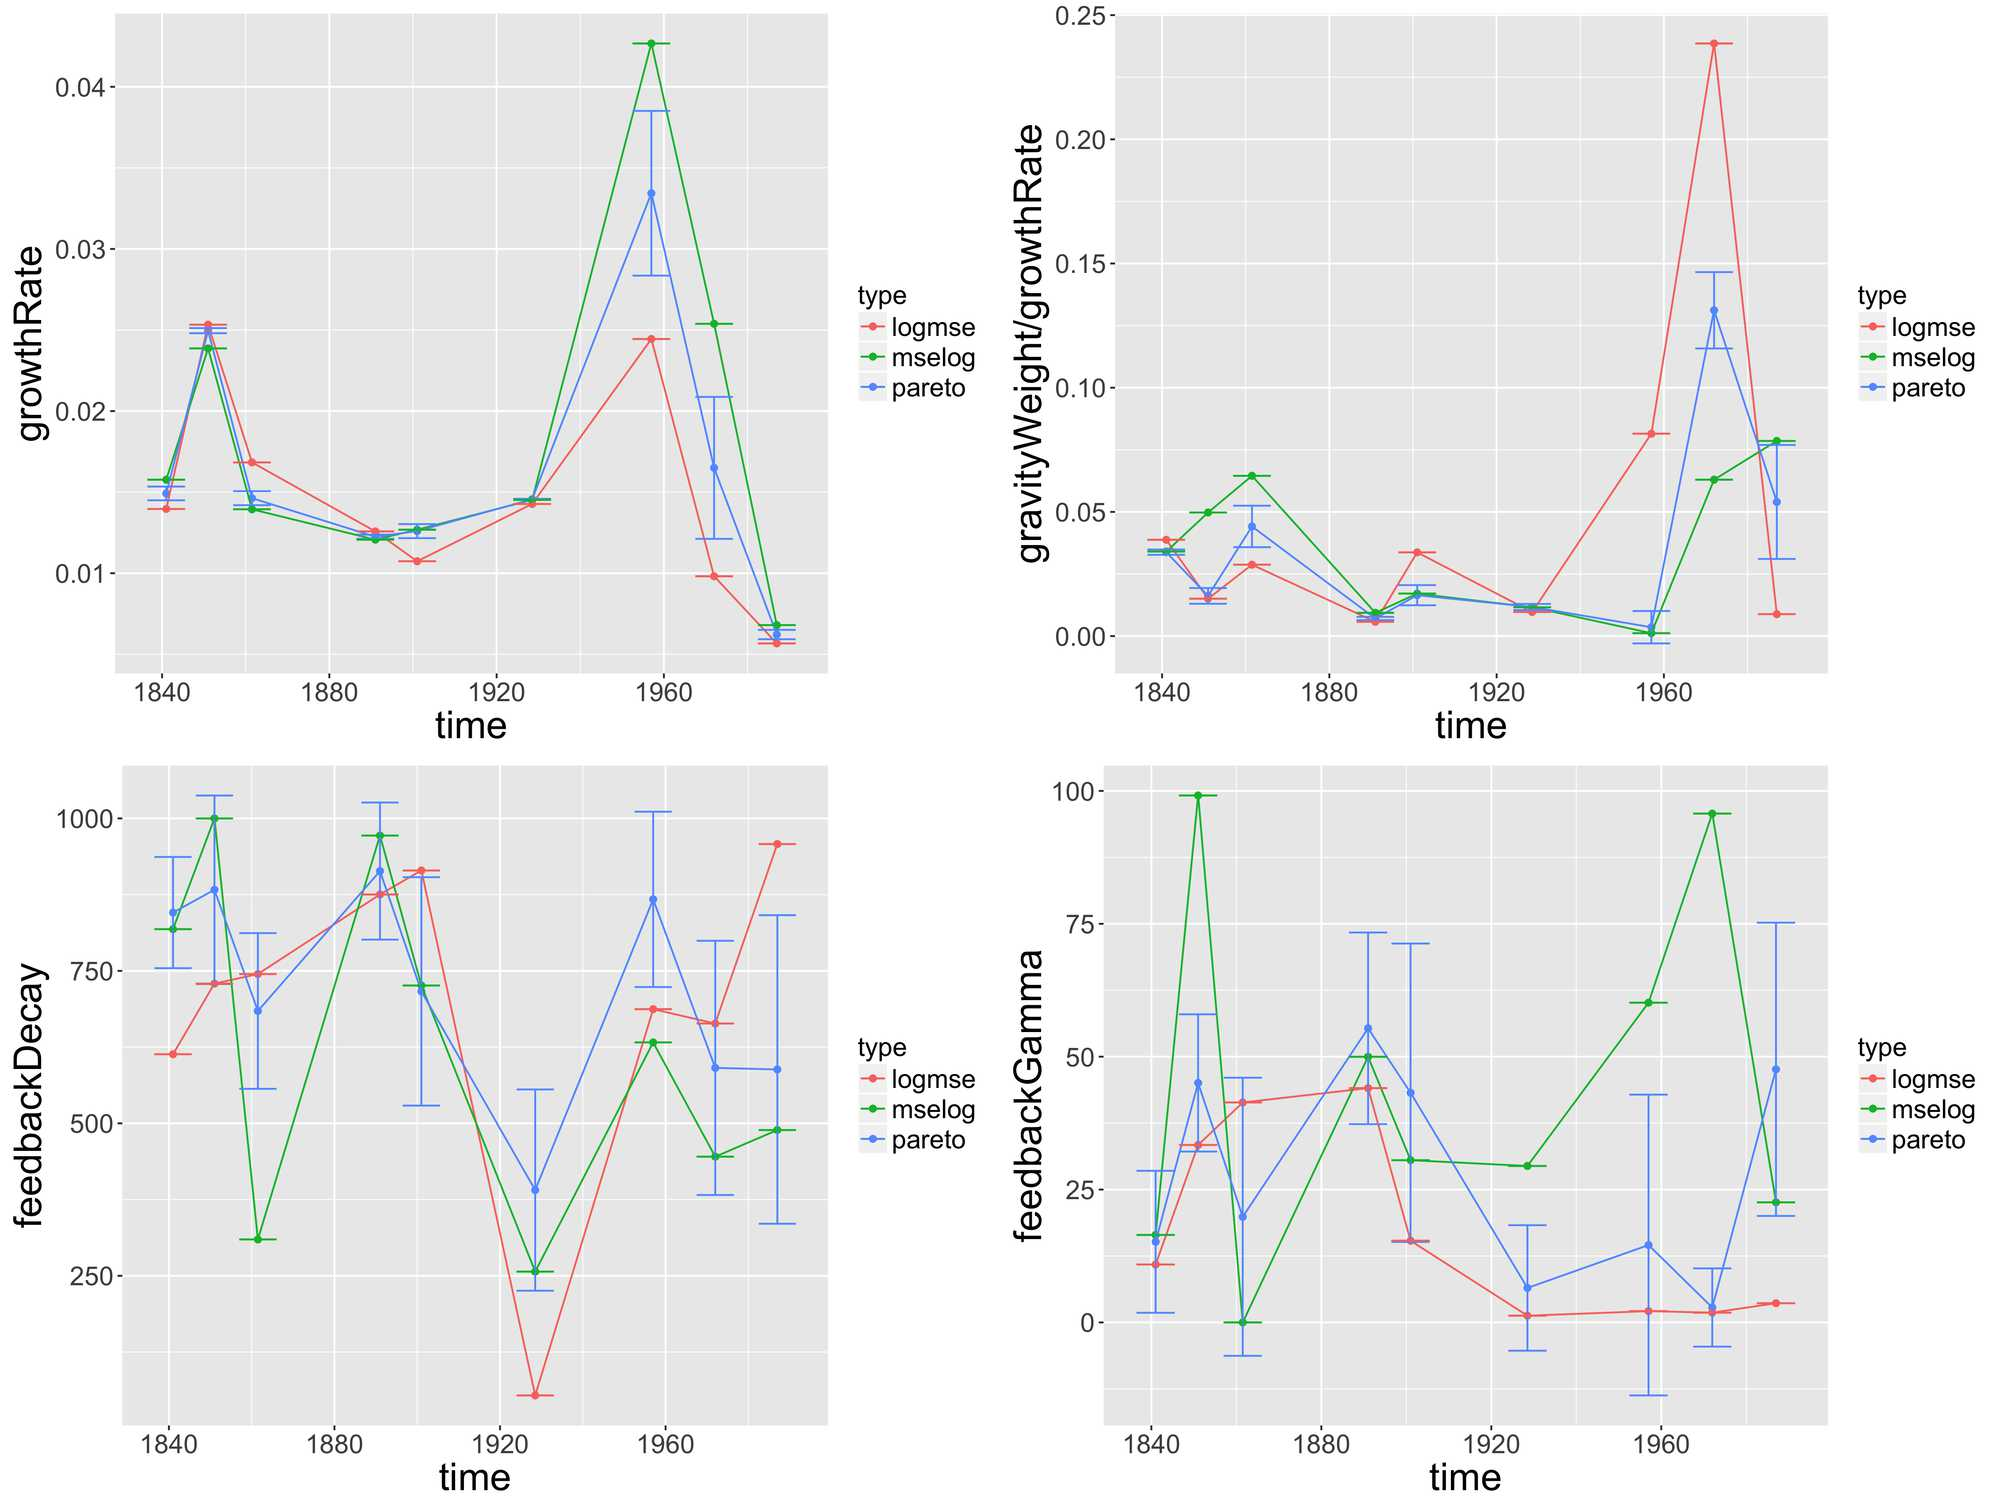
\includegraphics[width=\linewidth]{Figures/Final/4-3-2-fig-interactiongibrat-feedback}
\caption[Full model calibration][Calibration du modèle complet]{\textbf{Calibrated parameters for the full model.} We plot values of $r_0, w_G/r_0, d_N$ and $\gamma_N$ in time, for single-objective optimal points (Red and Green curves) and averaged over the Pareto front (Blue).\label{fig:interactiongibrat:feedback}}{\textbf{Paramètres ajustés pour le modèle complet.} Nous donnons les valeurs de $r_0, w_G/r_0, d_N$ et $\gamma_N$ dans le temps, pour les points optimaux pour les objectifs simples (courbes rouge et verte) et moyen sur le front de Pareto (bleu).\label{fig:interactiongibrat:feedback}}
\end{figure}
%%%%%%%%%%%%%%%%%%%%%%%%%%%







\paragraph{Estimating the compromise between fitting power and number of parameters}{Estimer le compromis entre puissance d'ajustement et nombre de paramètres}


\bpar{
We focus in this last experiment on quantifying the ``performance'' of the model, taking into account its predictive abilities, but also its structure. More precisely, we want to tackle the issue of overfitting, which has been for long recognized in Machine Learning for example~\cite{dietterich1995overfitting}, but for which there is a lack of methods for models of simulation. We need to introduce a tool to confirm that the improvement in model fit is not only artificially due to additional parameters.
}{
Nous visons dans cette dernière expérience à quantifier la ``performance'' du modèle, prenant en compte ses capacités prédictives, mais aussi sa structure. Plus précisément, nous voulons traiter la question de la surestimation (\textit{overfitting}), qui a été reconnue depuis un certain temps en Apprentissage Statistique par exemple~\cite{dietterich1995overfitting}, mais pour lequel il manque des méthodes applicables aux modèles de simulation\footnote{Cette question est en fait au coeur de la compréhension de la complexité : il s'agit de trouver une dimension qui capture la plus grande partie des dynamiques du système à un niveau donné, ce qui revient à déterminer un niveau de simplification qui capture les dynamiques agrégées, et donc l'émergence. Il pourrait d'ailleurs exister un lien entre cette question et ke problème de la détermination de l'\emph{embedding dimension} pour les séries temporelles, qui revient à trouver une dimension effective de l'espace des phases d'un système.}. Nous avons besoin d'introduire un outil qui confirme que l'amélioration de l'ajustement n'est pas uniquement artificiellement due aux paramètres supplémentaires. Cette étape est importante à ce stade d'introduction de modèles préliminaires : il s'agit en effet de construire des briques pertinentes mais également relativement simples.
}

\bpar{
The Akaike Information Criterion (AIC) provides for statistical models for which a likelihood function is available the gain in information between two models~\citep{akaike1998information}, correcting fit improvement for number of parameters. Similar methods include the Bayesian Information Criterion (BIC), which relies on slightly different assumptions and corrects differently. \cite{biernacki2000assessing} proposes an integrated likelihood as a generalization of these criteria in unsupervised classification. \cite{2017arXiv170108673P} shows that in the case of selecting the number of states in Hidden Markov Models, real cases induces too much pitfalls for standard methods to work robustly, and suggest pragmatic selection based on their results and expert judgement. In our case, the problem is that it is not even possible to define these.
}{
Le critère d'information d'Akaike (AIC) fournit pour les modèles statistiques pour lesquels une fonction de vraisemblance est disponible le gain d'information entre deux modèles~\cite{akaike1998information}, corrigeant l'amélioration du fit par le nombre de paramètres. Des méthodes similaires incluent le critère d'information Bayesien (BIC), qui repose sur des hypothèses légèrement différentes et corrige différemment. \cite{biernacki2000assessing} propose une likelihood intégrée comme une généralisation de ces critères pour la classification non-supervisée. \cite{2017arXiv170108673P} montre que dans le cas de la selection du nombre d'états pour des Modèles de Markov Cachés, les cas réels induisent trop d'embûches pour que les méthodes standard fonctionnement de manière robuste, et suggèrent une sélection pragmatique basée sur leurs résultats et le jugement d'expert. Dans notre cas, le problème est qu'il n'est même pas possible de les définir.
}


\bpar{
The method we propose is based on the intuitive idea of approaching models of simulation by statistical models and using the corresponding AIC under certain validity conditions. \cite{2017arXiv170609773B} uses a similar trick of considering the models as black boxes and approaching them to gain insights, in their case to extract interpretable structure as decision trees. Let $(X,Y)$ be the data and observations. We consider computational models as functions $(X,\alpha_k) \mapsto M_{\alpha_k}^{(k)}(X)$ mapping data values to a random variable. What is seen as data and parameters is somehow arbitrary but is separated in the formulation as corresponding dimensions will have different roles. We assume that the models have been fitted to data in the sense that an heuristic has been used to find an approximate optimal solution $\alpha^{\ast}_k = \argmin_{\alpha_k}\norm{M_{\alpha_k}^{(k)}(X) - Y}$, and we write $\varepsilon_k = \norm{M_{\alpha_k}^{(k)}(X) - Y}^2$ the corresponding mean-square error. For each optimized computational model, a statistical model $S^{(k)}$ with the same degree of freedom can be fitted on a set of realizations: $M^{(k)}_{\alpha^{\ast}_k}(X) = S^{(k)} (X)$, with an error $s_k = \norm{M_{\alpha^{\ast}_k}^{(k)}(X) - S^{(k)}(X)}^2$. If statistical models are good approximations of models compared to models discrepancy to reality, namely $s_k \ll \varepsilon_k$, then the gain of information between the two should mostly capture the gain of information between simulation models. We define therefore an \emph{Empirical AIC} measure between two simulation models by
}{
La méthode que nous proposons est basée sur l'idée intuitive d'approcher les modèles de simulation par des modèles statistiques et d'utiliser l'AIC correspondant sous certaines conditions de validité. \cite{2017arXiv170609773B} utilise une astuce similaire de considérer les modèles comme des boites noires et de les approcher pour gagner de l'information, dans leur cas pour extraire une structure interprétable sous forme d'arbres de décision. Soit $(X,Y)$ les données initiales et les observations des réalisation. Nous considérons les modèles computationnels comme des fonctions $(X,\alpha_k) \mapsto M_{\alpha_k}^{(k)}(X)$ faisant correspondre les valeurs des données à une variable aléatoire. Ce qui est vu comme données et comme paramètres est dans une certaine mesure arbitraire mais est séparé dans la formulation puisque les dimensions correspondantes auront des rôles différents. Nous supposons que les modèles ont été ajustés aux données au sens où une heuristique a été utilisée pour trouver une solution optimale approximative $\alpha^{\ast}_k = \argmin_{\alpha_k}\norm{M_{\alpha_k}^{(k)}(X) - Y}$, et nous écrivons $\varepsilon_k = \norm{M_{\alpha_k}^{(k)}(X) - Y}^2$ l'erreur carrée moyenne correspondante. Pour chaque modèle computationnel optimisé, un modèle statistique $S^{(k)}$ avec le même degré de liberté peut être ajusté sur un ensemble de réalisations : $M^{(k)}_{\alpha^{\ast}_k}(X) = S^{(k)} (X)$, avec une erreur $s_k = \norm{M_{\alpha^{\ast}_k}^{(k)}(X) - S^{(k)}(X)}^2$. Si les modèles statistiques sont de bonnes approximations des modèles en comparaison de la distance des modèles à la réalité, c'est à dire si $s_k \ll \varepsilon_k$, alors le gain d'information entre les deux devrait majoritairement capturer le gain d'information entre les modèles de simulation. Nous définissons ainsi une mesure d'\emph{AIC empirique} entre deux modèles de simulation par
}


\begin{equation}
I\left( M^{(1)}, M^{(2)}\right) = \Delta AIC \left[S^{(1)},S^{(2)}\right]
\end{equation}


%  M1 :
%  growthRate gravityWeight gravityGamma gravityDecay
%  0.01334922  0.0001287938      3.82252 401997651796
% logmse1 = 31.23745 ; mselog1 = 302.8934
%
%  M2 : 
% growthRate gravityWeight gravityGamma gravityDecay feedbackWeight feedbackGamma feedbackDecay
%  0.01283191  0.0001308851     3.809335 8.434855e+14      0.6034981 1.148056  7.474787e+14
% logmse2 =  31.2366040803222 ; mselog2 = 302.933997941623
%


\bpar{
In practice we calibrate the gravity only model and the full model on the full time span, and choose two intermediate solutions giving $M^{(1)}$ at $r_0=0.0133, d_G = 4.02e12, w_G = 1.28e-4, \gamma_G = 3.82$ with $\varepsilon_G=31.2375,\varepsilon_L=302.89$ and the full model $M^{(2)}$ at $r_0=0.0128, d_G = 8.43e14, w_G = 1.230e-4, \gamma_G = 3.81, w_N=0.60, d_N=7.47e14, \gamma_N = 1.15$ with $\varepsilon_G=31.2366,\varepsilon_L=302.93$. It is not clear how the empirical method is sensitive to the type of statistical model used, we use therefore severals for robustness, each time with the corresponding number of parameters (4 for the first and 7 for the second model): a polynomial model of the form $a_0 + \sum_{i>0} a_i X^i$, a mixture of logarithm and polynomial as $a_0 + a_1 \ln X + \sum_{i>1} a_i X^i$ and a generalized polynomial with real power coefficients that are optimized for model fit using a genetic algorithm $a_0 + \sum_{i>0} a_i X^{\alpha_i}$. We fit the statistical models using successive years as different realizations. Results for each are shown in Table~\ref{tab:interactiongibrat:empiricalaic}. We give the value of $s_k / \varepsilon_k$ and the $\Delta AIC$. We also provide the $\Delta BIC$ to check the robustness regarding the information criterion used. We find a positive value for 5 criteria out of 6, what means that information gain is indeed positive. The gain decreases when statistical model fit improves, and only the BIC for the optimized model fails to show an improvement. The assumption of negligible errors is always verified as the rate is always around 1\%. This approach is of course preliminary and further work should be done for a more systematic testing and more robust justification of the method. It suggests however that fit improvement in the model of simulation are effective, and that the model reveals therefore network effects.
}{
En pratique, nous calibrons le modèle de gravité seul et le modèle complet sur la période temporelle complète, et choisissons deux solutions intermédiaires donnant $M^{(1)}$ à $r_0=0.0133, d_G = 4.02e12, w_G = 1.28e-4, \gamma_G = 3.82$ avec $\varepsilon_G=31.2375,\varepsilon_L=302.89$ et le modèle complet $M^{(2)}$ à $r_0=0.0128, d_G = 8.43e14, w_G = 1.230e-4, \gamma_G = 3.81, w_N=0.60, d_N=7.47e14, \gamma_N = 1.15$ avec $\varepsilon_G=31.2366,\varepsilon_L=302.93$. Il n'est pas clair dans quelle mesure la méthode empirique est sensible au type de modèle statistique utilisé, nous utilisons pour cela un certain nombre pour la robustesse, à chaque fois avec les nombre de paramètres correspondants (4 pour le premier et 7 pour le second modèle) : un modèle polynomial de la forme $a_0 + \sum_{i>0} a_i X^i$, une mixture de logarithme et polynôme comme $a_0 + a_1 \ln X + \sum_{i>1} a_i X^i$ et un polynôme généralisé avec des exposants réels qui ont été optimisés pour la performance du modèle par utilisation d'un algorithme génétique $a_0 + \sum_{i>0} a_i X^{\alpha_i}$. Nous ajustons les modèles statistiques en utilisant les années successives comme des réalisations différentes. Les résultats pour chaque sont donnés en Table~\ref{tab:interactiongibrat:empiricalaic}. Nous donnons les valeurs de $s_k / \varepsilon_k$ et le $\Delta AIC$. Nous donnons aussi le $\Delta BIC$ pour vérifier la robustesse au regard du critère d'information utilisé. Nous trouvons une valeur positive pour 5 critères sur 6, ce qui signifie que le gain d'information est effectivement positif. Le gain décroît quand la performance du modèle statistique augmente, et seul le BIC pour le modèle optimisé échoue à montrer une amélioration. L'hypothèse des erreurs négligeables est toujours vérifiée puisque le taux est toujours autour de 1\%. Cette approche est bien sûr préliminaire et des développements supplémentaires seraient nécessaires pour un test plus systématique et une justification plus robuste de la méthode. Cela suggère cependant que l'amélioration de fit dans le modèle de simulation sont effectifs, et que le modèle révèle par cela des effets de réseau.
}


%\comment[JR]{revoir possible alternatives empiriques : TIC ? \cite{burnham2003model}}

%\comment{revoir comparabilité entre differents datasets : akaike weights ?}
% https://www.sciencedirect.com/science/article/pii/B9780125893206500204
% https://stats.stackexchange.com/questions/32511/using-aic-to-distinguish-between-models-using-multiple-datasets
% http://onlinelibrary.wiley.com/doi/10.1901/jeab.2007.01-06/epdf

% lien avec l'embedding dimension possible ?
% rq : au coeur de la complexité : overfitting ~ dimension effective -> a quel moment des interactions micro creent un attracteur a un niveau agrege = emergence !
% http://www.sciencedirect.com/science/article/pii/S016727899800089X



% \comment[FL]{pour info je n'ai pas lu en detail : masi ca m'a l'air bien ciblé}


%%%%%%%%%%%%%%%%%%%%%%%%
\begin{table}[ht]
\caption[Empirical AIC values][Valeurs de l'AIC empirique]{Empirical AIC results.}{Valeurs de l'AIC empirique.\label{tab:interactiongibrat:empiricalaic}}
\begin{tabular}{|l|l|l|l|l|l}
\hline
Modèle Statistique & Ajustement pour $M^{(1)}$ & Ajustement pour $M^{(2)}$ & $\Delta AIC$ & $\Delta BIC$\\
\hline
Polynomial & 0.01438 & 0.01415 & 19.59 & 3.65\\
Log-polynomial & 0.01565  & 0.01435 & 125.37 & 109.43\\
Polynomial Généralisé & 0.01415  & 0.01399 & 11.70 & -4.23\\
\hline
\end{tabular}
\end{table}
%%%%%%%%%%%%%%%%%%%%%%%%







\subsection{Towards co-evolutive models}{Vers des modèles co-évolutifs}


\bpar{
Our focus on network effects remains quite limited since (i) we do not consider an effective infrastructure but abstract flows only, and (ii) we do not take into account the possible network evolution, due to technical progresses~\citep{bretagnolle2000long} and infrastructure growth in time. An interesting development would be first the application of our model with real network data, using effective distance matrices in time, computed e.g. with the train network used by~\cite{thevenin2013mapping}. Then, allowing the network to dynamically evolve in time, as a function of flows, would yield a model of co-evolution between cities and transportation networks for a system of cities, which has been proven empirically by~\cite{bretagnolle:tel-00459720}. This kind of model is very rare, and \cite{schmitt2014modelisation} provides with SimpopNet one of the few examples. It is shown by \cite{raimbault2016models} that disciplinary compartmentalization may be at the origin of the relative absence of such type of models in the literature. Indeed, it would imply to include heterogenous processes such as economic rules to drive network growth, that are quite far from the approach taken. It would however allow to investigate to what extent the refinement of network spatial structure and network dynamics can improve the explanation of urban system dynamics.
}{
Rappelons le positionnement de l'étude que nous venons de mener par rapport à notre objectif général. Notre compréhension des effets de réseau reste ici assez limitée puisque (i) nous ne considérons pas une infrastructure réelle mais uniquement des flux abstraits, et (ii) nous ne prenons pas en compte la possible évolution du réseau, due aux progrès techniques~\cite{bretagnolle2000long} et à la croissance de l'infrastructure dans le temps. Un développement intéressant sera d'abord l'application du modèle sur des données réelles de réseau, en utilisant les matrices de distance réelles dans le temps, calculées e.g. avec le réseau ferré utilisé par~\cite{thevenin2013mapping}. Ensuite, permettre au réseau d'évoluer de manière dynamique dans le temps, comme fonction des flux, produira un modèle de co-évolution entre les villes et les réseaux de transport pour un système de villes, qui a été prouvée empiriquement par~\cite{bretagnolle:tel-00459720}. Ce type de modèle est très rare, et \cite{schmitt2014modelisation} fournit avec SimpopNet l'un des exemples. Il est montré dans la section~\ref{sec:quantepistemo} que la séparation des disciplines pourrait être à l'origine de l'absence relative de tels types de modèles dans la littérature. En effet, cela impliquerait d'inclure des processus hétérogènes comme des règles économiques pour régir la croissance du réseau, qui sont assez loin de l'approche prise. Cela permettrait cependant d'investiguer dans quelle mesure le raffinement de la structure spatiale du réseau et des dynamiques de réseau peut améliorer l'explication des dynamiques des systèmes urbains. La pertinence d'un tel développement est confirmée par les approches empiriques, comme~\cite{dupuy1996cities} qui montre le rôle de la position des villes dans le réseau autoroutier Européen pour leur relations respectives et leur compétitivité. 
}


\bpar{
We have introduced a spatial model of growth for a system of cities at the macroscopic scale, including second order network effects among endogenous growth and direct interaction growth drivers. The model is parametrized on real data for the French city system between 1831 and 1999. The calibration of the model in time provides interpretations for the evolution of processes of interaction within the system of cities. We furthermore show that the model effectively unveils network effects by controlling for overfitting. This work paves the way for more complicated models with dynamical networks, that would capture the co-evolution between transportation network and territories.
}{
Nous avons introduit un modèle spatial de croissance pour un système de villes à l'échelle macroscopique, incluant des effets de réseau au second ordre avec la croissance endogène et les interaction directes comme moteurs de la croissance. Le modèle est initialisé sur les données réelles du système de villes français entre 1831 et 1999. La calibration du modèle dans le temps fournit des interprétations pour l'évolution des processus d'interaction dans le système de villes. Nous montrons de plus que le modèle révèle effectivement des effets de réseau en contrôlant l'overfitting. Ce travail ouvre la voie pour des modèles plus compliqués avec des réseaux dynamiques, qui captureraient la co-évolution entre les réseaux de transport et les territoires, qui seront développés au Chapitre~\ref{ch:macrocoevolution}.
}






\stars








